\documentclass{article}

\title{Geonomics: A Python package for building agent-based, spatially explicit, and arbitrarily complex landscape-genomic and spatial-ecology simulations}
\author{Drew Hart}
\date{January 18, 2019}

%%%%%%%%%%%%%%%%%%%%%%%%%%%%%%%%%%%%%%%%%%%%%%%%%%%%%%%%%%%%%%
% TODO:
% 1] mention WHY I chose each validations test (i.e. which components of Geonomics it tests/demonstrates

% 2] perhaps think through the meaning/implications of the details of the Yosemite example soome more, perhaps change some parameters (e.g.\ emulate some specific species; treat each timestep as a year and simulate just 100 years and a realistic amount of temperature change
% during that time; parameterize the fitness cost from field data?), and/or perhaps
% run two or a few distinct scenarios (maybe where the species varies in mobility), to
% see if potential to adapt depends on movement (and hence on gene flow capacity)?
% or perhaps run the same model twice, with the difference being that the environmental change takes place over 1000 timesteps in the first model, but only 100 in the second?

% 3] fix the means by which the Yosemite raster is read in and normalized and used for a 
% Landscape Layer, a K raster, etc; change all of these to raster files that are
% pointed to in the params file and read in from file by Geonomics (as explained in the
% text below

% 4] add the timestep flow diagram

%%%%%%%%%%%%%%%%%%%%%%%%%%%%%%%%%%%%%%%%%%%%%%%%%%%%%%%%%%%%%%

% load packages
\usepackage{graphicx} % to include graphics
\usepackage{url}      % to include URLs
\usepackage{fullpage} % use 1-inch margins
\usepackage{amsmath}  % for creating equations
\usepackage[font=footnotesize, labelfont=bf]{caption}  % create figure captions

% create typewriter environment
\newenvironment{allintypewriter}{\ttfamily}{\par}


\begin{document}

\maketitle

\section{Abstract}

{\LARGE TO BE COMPLETED}


\section{Intro/Background}
There is ever-growing interest in understanding and even predicting
the genomic evolution of complex study systems. 
These systems often feature one or multiple populations or species that are not
at equilibrium, that inhabit complex and even changing landscapes, and that are 
undergoing both neutral evolution and natural selection (often on multiple traits).

The complex genomics of such systems are beyond the reach of analytical
population genetics. The spatial context and non-neutral evolutionary
dynamics of these systems make them intractable for coalescent simulation.  
Yet study systems such as these are ever more important for our understanding
of evolutionary biology, environmental management and conservation, and the
implications of climate change, urbanization, and other anthropogenic
environmental changes.

Modern population genetics has very few tools that can approach
such systems in their full complexity. Most simulation packages are lacking
at least one of numerous important features---selection on an arbitrary traits
with complex genomic architectures, realistic recombination,
realistic movement in a spatially explicit environment,
environmental and demographic change 
{\large cite SimAdapt, cdpop, quantiNemo, etc}---and the few tools that approach
this level of complexity have a very high cost of admission
(e.g.\ considerable programming skill, or even ithe requirement
that the user to learn a new, custom-made programming language
{\large cite Messer: SLiM}). 

Additionally, empirical studies often use sophisticated statistical methods
to make inferences or predictions about the evolutionary history,
dynamics, or future of wild populations (e.g.\ adaptive potential
{\large cite VARIOUS STUDIES HERE}; genomic vulnerability index
{\large citeYELLOW WARBLER STUDY}). Yet we have no well established evolutionary
null model, and thus a limited understanding of the neutral genomic expectations
and Type-II error rates of genomic outlier tests in such systems. Adequately
complex simulations can help calibrate statistical analyses in these cases.

Thus there is clear need for broad-purpose, flexible software for
landscape-genomic simulation.
Such software should be hosted in a
popular scripting language, and should allow the user to build complex
models with minimal programming expertise, but it should offer deep
customizability to the advanced user.
Geonomics aims to meet this need.


\section{Model overview}

Geonomics builds agent-based, forward-time, spatially explicit simulations
for landscape-genomic and spatial-ecology scenarios of arbitrary complexity.
Users can simulate one or many species (i.e.\ reproductively isolated populations)
on landscapes with any number of layers (i.e.\ environmental variables)
from artificial or real-world rasters.
Users create their models by first generating, editing, and then processing
a Geonomics parameters file.

Each species is described by a wide variety of import life-history traits that
determine its behavior (e.g.\ intrinsic growth rate, mate-search radius, mean number of
offspring per mating event, reproductive age and maximum age, etc;
see the documentation for a detailed discussion of each parameter).
A species can also use a number of optional features
and activities---movement; demographic- and life-history change events;
and diploid, biallelic genomes determined by a genomic architecture
with zero or more monogenic or polygenic traits
and with or without neutral, deleterious, and trait mutations.
(Note that Geonomics models can actually be built and run without using genomes at all,
e.g.\ for use in movement-ecology simulations,
even though genomic simulation is clearly at
the heart of its inspiration and design.)

Each layer can be used to determine a number of the characteristics and behaviors of a
species, including its spatially explicit carrying capacity;
its movement and/or dispersal across the landscape (note that Geonomics 
uses the term `movement' to refer to the movement of individuals of non-sessile species,
and uses the term `dispersal' exclusively to refer to the dispersal of offspring from 
their parents' midpoint at the time of the offspring's birth); and the environmental
variable that serves as the selective force for each of a species' traits. A layer
can also be parameterized to go through any number of change events (each one starting
and finishing at pre-determined timesteps, and proceeding stepwiseat between them
at pre-determined intervals).

A model can be run for any number of timesteps. Each timestep has a fixed schedule
of operations, which are depicted in fig. 1. The timestep starts by updating the
model's timestep counter, updating all individuals' ages, and updating each species'
population-size record. Then each species, if it is not sessile, undergoes movement. 

Movement is in continuous space, with individuals' distances
and directions drawn separately then composed into movement vectors. Directions can be
drawn from a uniform distribution on the unit circle, resulting in isotropic movement
(the default behavior); alternatively, they can be drawn from an array
of unimodal or multimodal Von Mises distributions superimposed on
a landscape layer (serving as a conductance surface from which the distributions
are derived), resulting in anisotropic movement that simulates realistic movment 
across an environment of heterogenous habitat quality.

After movement completes, then each species mates.
Mating pairs are chosen from among all pairs of 
individuals within the species' mate-search radius
(based on eligibility by age and sex, and a Bernoulli draw with probability equal
to the species' intrinsic birth rate), and for each mating pair a number of offspring
is chosen (from a Poisson distribution with lambda equal to the species' mean number
of offspring). Each offspring is dispersed to a new location; as with movement, dispersal
is in continuous space, with direction drawn either isotropically or
anisotropically. And if the species uses genomes, then each offspring has a new genome
assigned to it, which is the fusion of two gametes, one from each parent, which are
generated according to Mendelian principles and with realistic recombination (according
to the array of recombination rates in the species' genomic architecture).

Mating is followed by mortality. Individuals' death probabilities result from
a combination of their probability of death by density-dependence (which is
operationalized by a spatialized logistic-growth model; see section
\emph{\texttt{Community}, \texttt{Species}, and \texttt{Individual}} for details)
and their probability of death by natural selection (which can operate on any number
of traits simultaneously; see section
\emph{genomes, \texttt{GenomicArchitecture}, and \texttt{Trait}} for details). 

Finally, any of a number of optional operations are carried out. These include
landscape-change events, species-change events (be they demographic changes or
changes to key life-history parameters), and collection of data and statistics.

When a model is created, its landscape is seeded randomly with a chosen number of
starting individuals for each species. When the model is first run it goes through an
indeterminate burn-in phase (without genomic data), which ends as soon as a set of
threshold-decision checks passes successfully, indicating that the species has
reached a dynamic equilibrium in population size and distribution.
After the burn-in, for each species, if genomes are to be used then a genome is drawn
(in accordance with how the species' genomic architecture was parameterized)
and assigned to each individual.
Then the model's main phase can run for any number of steps; at the scheduled
timesteps, it will carry out any species- and landscape-change events,
and will save the required data and/or statistics
(in a directory-tree organized by iteration, species, then file content).

Once a model is built, the user can either choose to run it to completion (i.e.\ for its
parameterized number of timesteps, for its parameterized number of iterations) or to
run it manually for any number of timesteps (stopping intermittently, if needed, to
introspect the model, collect custom data, or make manual alterations).

{\large INCLUDE SINGLE-TIMESTEP FLOW DIAGRAM}


\section{Design, Structure, and Function}
Geonomics is designed to allow the creation of complex, highly customizable
landscape-genomic simulation models with a minimal amount of programming work or even
programming experience.
After launching Python and loading the package (\texttt{>>> import geonomics as gnx}),
for the simplest use-case (see fig. 1), the user need only:
\begin{enumerate}
        \item execute a command to create a template parameters file (`gnx.make\_parameters\_file(\ldots)`), feeding in the necssary arguments (see the command's documentation for details);
        \item edit the parameters file as desired;
        \item execute a command to make a \texttt{Model} object from parameters file (`mod = gnx.make\_model(\ldots)`);
        \item execute a command to run the model to completion (`mod.run(\ldots)`).
\end{enumerate}

% fig 1
\begin{figure}[h!]
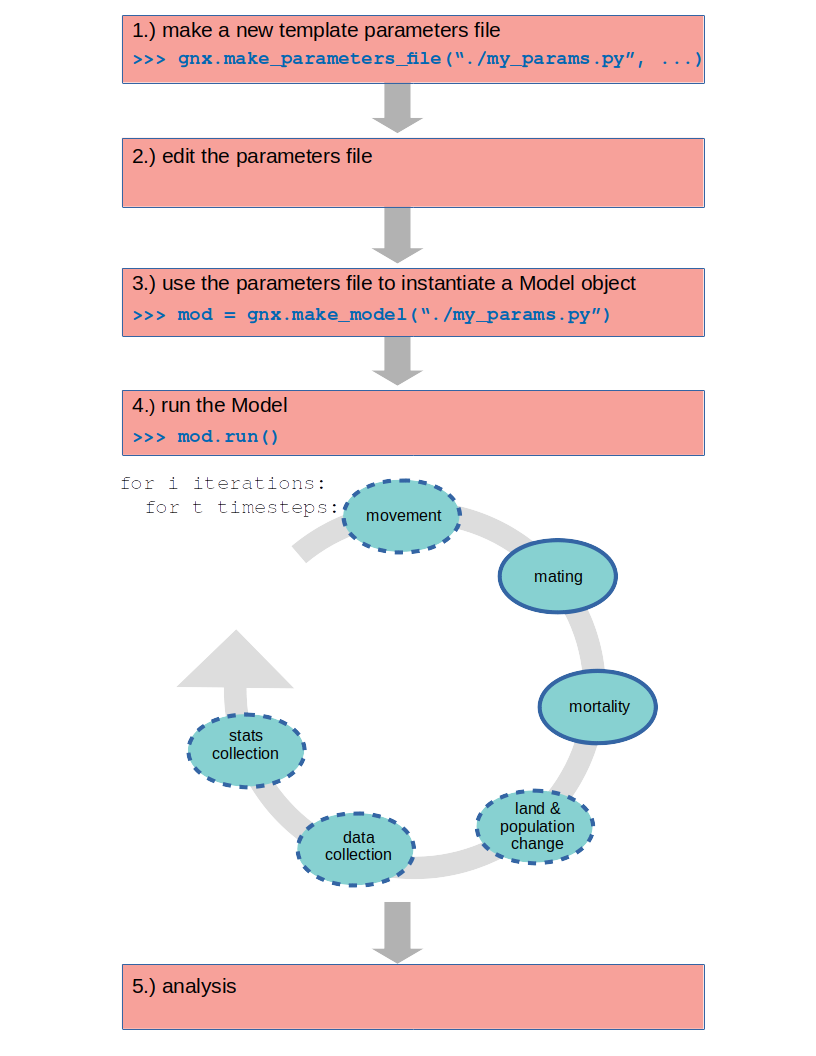
\includegraphics[width=125mm]{./img/flow_diagram.png}
\caption{Geonomics flow diagram}
\end{figure}

In more complicated use-cases, the user may wish to use the `mod.walk(\ldots)`
command to run the model for a limited number of timesteps,
and to intercalate any of the above steps with their own code
(to manually edit the Model object, and/or collect data from the \texttt{Model} before or
during the run).

Python is an excellent language for object-oriented programming,
and this is the predominant paradigm in which Geonomics is written.
This means that the core data structures with which the user will interface
are objects belonging to classes defined by Geonomics.
The following paragraphs provide a brief review of the major and minor classes, including
what data they contain and what they do. (For full details, see the Geonomics
documentation: \url{http://htmlpreview.github.io/?https://github.com/drewhart/geonomics\_docs/blob/master/built/doc.html}.)


\subsection{\texttt{Model}}
The \texttt{Model} class is the topmost class of the package.
A \texttt{Model} object contains the landscape and species of a model and a copy of the
parameters used to create the \texttt{Model}.
It runs each timestep of a simulation by implementing, in the following order,
if and when applicable: movement; mating and dispersal; mortality;
landscape changes; species changes; and collection of data and statistics.
As simulations run, the \texttt{Model} object tracks the timesteps and iterations.
The user can call functions that belong to the \texttt{Model}, also known as methods,
by using Python's dot notation (e.g.\ the \texttt{Model} can be run to completion using
the \texttt{run} function, which can be called as \texttt{mod.run()},
where \texttt{mod} is a \texttt{Model}
object). The \texttt{Model} object also offers numerous plotting methods, for exploring,
debugging, and presenting simulations.


\subsection{texttt{Landscape} and \texttt{Layer}}
The \texttt{Model.land} attribute contains an instance of the \texttt{Landscape} class.
This class is a Python \texttt{dict} containing serial integer-keyed instances of the
\texttt{Layer} class. Each \texttt{Layer} represents, as the name implies, a single,
coregistered raster layer on the landscape, and contains the actual raster data itself
in the \texttt{Layer.rast} attribute (as a `\texttt{numpy.ndarray}, an array belonging to the
Python package \texttt{numpy}).


\subsection{\texttt{Community}, \texttt{Species}, and \texttt{Individual}}
The \texttt{Model.comm} attribute contains an instance of the \texttt{Community} class.
This class is a \texttt{dict} of serial integer-keyed instances of the 
\texttt{Species} class. 
While most simulations will probably only involve a single \texttt{Species},
the \texttt{Community} provides the option for including multiple 
\texttt{Species} in a single simulation.
This creates the potential for implementing inter-species interactions (which future
versions of Geonomics may include).

Each \texttt{Species} is a \texttt{dict} of serial integer-keyed \texttt{Individual}
objects.
The \texttt{Species} object has a number of important attributes controlling
model behavior, including: the current population-density raster
(attribute \texttt{Species.N});
the intrinsic population growth rate (attribute \texttt{Species.R});
the carrying-capacity raster (attribute \texttt{Species.K}, which is used in
the spatialized logistic-growth model that controls population growth and density); 
optionally, a \texttt{GenomicArchitecture} object, which defines the
neutral and adaptive genomic features of the species and tracks all mutations that occur
(attribute \texttt{Species.gen\_arch}; described below);
and optionally, objects of the \texttt{\_MovementSurface} and/or
\texttt{\_DispersalSurface classes}, which can use arrays of unimodal or multimodal
Von Mises distributions to implement non-isotropic movement or dispersal across a
\texttt{Layer}'s raster (private attributes \texttt{Species.\_move\_surf} and
\texttt{Species.\_disp\_surf}).
(Importantly, while the name of the \texttt{Species} class implies that
it models only species, it would be possible for the user to use the class to model
subspecies, subpopulations, or incipient species, for example, were appropriate
home-brewed code to regulate the possibility for inter-\texttt{Species} mating events
and/or other interactions.)

Each \texttt{Individual} has a number of descriptive attributes. These include
x- and y-coordinates on the Landscape (attributes \texttt{Individual.x}
and \texttt{Individual.y}); age and sex (attributes \texttt{Individual.age} and
\texttt{Individual.sex}); current environmental values (extracted from the
\texttt{Landscape} cells within which the \texttt{Individual} is currently located;
attribute \texttt{Individual.e}); optionally, a genome (attribute
\texttt{Individual.g}, described below); and optionally, phenotypes for each
\texttt{Trait} (attribute \texttt{Individual.z}; described below).

At each timestep, each \texttt{Individual}'s probability of death by density-dependence
is calculated as:

\begin{equation}
\begin{split}
       P(d_{x,y}) = E[N_{d;x,y}]/N_{x,y} = \frac{E[N_{b;x,y}] - \frac{\mathrm{d}N_{x,y}}{\mathrm{d}t}}{N_{x,y}}
\end{split}
\end{equation}

where $E[N_{d;x,y}]$ is the expected number of deaths at position x,y on the
\texttt{Landscape}; $N_{x,y}$ is the population density at position x,y;
$E[N_{b;x,y}$ is the expected number of births at position x,y;
and $\frac{\mathrm{d}N_{x,y}}{\mathrm{d}t}$ is the
logistic population growth rate at position x,y.


\subsection{genomes, \texttt{GenomicArchitecture}, and \texttt{Trait}}
As mentioned in the previous section, when genomes are used, each \texttt{Individual} has
a genome saved in the \texttt{Individual.g} attribute. Genomes are not implemented
as a special Geonomics class; rather, they are simply Lx2 binary \texttt(numpy) arrays,
(L is the length of the genome, or the number of loci simulated; 2 because genomes
are diploid; binary because all loci are biallelic).

Genomes are realistically, biparentally inherited. But the original genomes used to
initiate the starting population are randomly assigned in accordance with the
\texttt{Species}' \texttt{GenomicArchitecture}. The \texttt{GenomicArchitecture} defines
a number of genomic features, including:
\begin{itemize}
        \item the length of the simulated genome (attribute \texttt{GenomicArchitecture.L});
        \item the starting allele frequencies at all loci (attribute \texttt{GenomicArchitecture.p});
        \item the recombination rates between all loci (attribute \texttt{GenomicArchitecture.r});
        \item the dominance flags for all loci (attribute \texttt{GenomicArchitecture.dom});
        \item a record of all non-neutral loci (attribute \texttt{GenomicArchitecture.nonneut\_loci}).
        \item the neutral, deleterious, and trait mutation rates (attributes \texttt{GenomicArchitecture.mu\_neut} and \texttt{GenomicArchitecture.mu\_delet} and the attribute \texttt{Trait.mu}, described below);
        \item the genomic architecture of all \texttt{Trait} objects (attribute \texttt{GenomicArchitecture.traits}; described below);
        \item other secondary data (see documents for details).
\end{itemize}

The \texttt{GenomicArchitecture.traits} attribute is a \texttt{dict} of serial
integer-keyed \texttt{Trait} objects, one for each trait that is simulated for the
corresponding \texttt{Species}. Each \texttt{Trait} object defines all requisite
information for the trait it parameterizes, including:
\begin{itemize}
        \item the number of loci underlying the trait (attribute \texttt{Trait.n\_loci});
        \item the indices of the loci underlying the trait (attribute \texttt{Trait.loci});
        \item the effect sizes, i.e.\ $\alpha$ values, of all loci underlying the trait (attribute \texttt{Trait.alpha});
        \item the parameters controlling the distribution from which the effect sizes of the trait's loci are drawn (attributes \texttt{Trait.alpha\_distr\_mu} and \texttt{Trait.alpha\_distr\_sigma});
        \item the mutation rate for the trait (attribute \texttt{Trait.mu});
        \item the trait's polygenic selection coefficient (or array of selection coefficients, should selection-strength vary spatially) i.e.\ $\phi$ (which for a monogenic trait is equivalent to the selection coefficient \emph{s} in classic population-genetic literature; attribute \texttt{Trait.phi});
        \item other information (see documentation for details).
\end{itemize}

For each trait, each \texttt{Individual}'s phenotype is calculated as:

\begin{equation}
z_{i;p} = null\_genotype + \sum_{l = 0}^{n} \alpha_{p,l} g_{i,l}
\end{equation}

where $i$ is the \texttt{Individual}'s index, $p$ is the \texttt{Trait}'s index,
$n$ is the number of loci, $\alpha$ is a locus' effect size, $g$ is an
\texttt{Individual}'s genotype, and $null\_genotype$ is 0 for monogenic traits,
0.5 for polygenic traits. For each \texttt{Trait}, each \texttt{Individual}'s
phenotype then combines with their current x,y position to determine their
current absolute fitness as:

\begin{equation}
\omega_{i,p}= 1 - \phi_{p;x,y} (\mid e_{p;x,y} - z_{i;p} \mid)^{\gamma_{p}}
\end{equation}

where $\phi_{p;x,y}$ is the selection coefficient on \texttt{Trait} $p$ at the
\texttt{Individual}'s location; $e_{p;x,y}$ is the environmental value
of the \texttt{Layer} upon which selection operates for \texttt{Trait} $p$,
and $\gamma_{p}$ defines the curvature of the fitness function for \texttt{Trait} $p$.
The resulting fitness values, for all \texttt{Trait}s, function into each
\texttt{Individual}'s probability of death at each timestep by:

\begin{equation}
P(d_{i}) = 1 - (1 - P(d_{x,y})) \prod_{p = 1}^{m}\omega_{i,p}
\end{equation}

where $P(d_{x,y})$ is the \texttt{Individual}'s probability of death by
density-dependence (described above), and $m$ is the number of \texttt{Trait}s
the \texttt{Species} has.


\section{Validations tests}
Geonomics is designed to enable theoretical, methodological, empirical, and applied
research on complex evolutionary scenarios that are intractable (or inconvenient)
to simulate with existing software.
To garner trust in the data it simulates under such scenarios, 
it is imperative to first validate its behavior is valid under simpler,
well established population-genetic and population-genomic scenarios.
For this reason, this section walks through a series of six statistical
and heuristic validations tests, selected from among the most
common population-genetic models with an eye toward demonstrating the range
of functionality Geonomics offers.
I comprehensively demonstrate that Geonomics yields the expected results
for all of these models.
(The source code for all of these tests is available within the
\./tests/validation/ directory of the Geonomics repository.
Note that in some cases the code is quite extensive, given that these tests
emulate aspatial and spatially-implicit models using software designed to
create complex, spatially-explicit models; these classic population-genetic models
serve as excellent validations of the behavior of Geonomics,
but would in reality be much better served by simpler simulators.)


\subsection{Wright-Fisher test: genetic drift}
The Wright-Fisher model of genetic drift models a fixed-size haploid population that
turns over completely at each timestep (i.e.\ generation). The population can have
any number of independent, biallelic genetic loci (often symbolized as ‘A’ and ‘a’,
but symbolized as ‘0’ and ‘1’ in Geonomics). For each locus, each generation’s allele
frequency is chosen as a binomial random variable, with the number of draws equal to
the population size and the probability of drawing the ‘1’ allele equal to the previous 
generation’s ‘1’-allele frequency. The mean persistence time for an allele 
(i.e.\ the expected number of generations for which a locus remains segregating) 
is:

\begin{equation}
\bar{t}(p) = -4N[(1 - p)ln(1 - p) + pln(p)]
\end{equation}

where $2N$ is the number of alleles in the population (such that $N$ can
represent the diploid population size) and $p$ is the frequency of either allele
at the locus {large cite Hartl and Clark 2007}

Clearly, the Wright-Fisher model is much simpler than the sorts of models for which
Geonomics is designed (as are all of the following validations tests)---it is aspatial,
panmictic, features fixed population sizes, models only neutral loci, and so forth. 
I parameterized Geonomics so as to approximate the model as closely as possible.
To emulate aspatiality and panmixia, I used a population on a homogeneous landscape,
with isotropic movement, and with movement and dispersal distributions
and a mating radius that broadly encompass the diagonal width of the landscape.
To enforce complete generational turnover, I set the
maximum age parameter to 1 timestep. While Geonomics cannot maintain constant population
size, I maintained the carrying-capacity raster at a constant, uniform value, thus
maintaining a stationary mean population size. I simulated 100, independent neutral
loci (by setting all interlocus recombination rates to 0.5), with starting '1'-allele
frequencies of 0.5 (although the actual starting frequencies vary slightly around
this value because of sampling error when all individuals' genotypes are drawn binomially).
Of course, I did not implement natural selection or any environmental
or demographic changes.
(I set other parameter values reasonably, or left them at defaults;
see \texttt{wf\_params.py} for specifics.)


I ran the Wright-Fisher approximation test for three cell-values of the
carrying-capacity raster (i.e.\ three values of `K\_factor'), hence for three mean
population sizes. For each mean population size (calculated as the harmonic mean,
to account for stochastic fluctations around the carrying capacity), I compared
the mean persistence time to that
expected by theory, according to the formula cited in the previous paragraph. As can be
seen in figures 2 and 3, the results compare favorably to theory, although the observed
mean persistence time undershoots the expected at all population sizes because of a variety
of artefacts of the approximation. Despite the movement, dispersal, and mating-radius
parameterizations, the simulated populations will still exhibit some neighborhood-mating
behavior, generating a spatialized coalescent that reduces effective population size
below the harmonic mean of the census size. 
Effective population size should also undershoot harmonic-mean size in
Geonomics models because of the imperfection with which the "infinite gametes" assumption
of the Wright-Fisher model's binomial draws of allele frequencies is modeled by
random draws of alleles from each pair of mating parents. DOES THAT MAKE SENSE\ldots? Other
factors that would artificially reduce the time to fixation or loss of an allele include
the fact that most alleles are not starting off at precisely 0.5 frequencies; and the fact
that Geonomics uses a large, \emph{a priori} sample of genome-wide recombination events
to approximate realistic recombination at the stipulated recombination rates, such that
sampling error could lead to artificially inflated linkage between some neighboring pairs
of loci. Thus, overall, Geonomics demonstrates realistic Wright-Fisher-type drift, with
persistence times characteristic of a population whose effective size undershoots its
mean size.

% fig 2
\begin{figure}[h!]
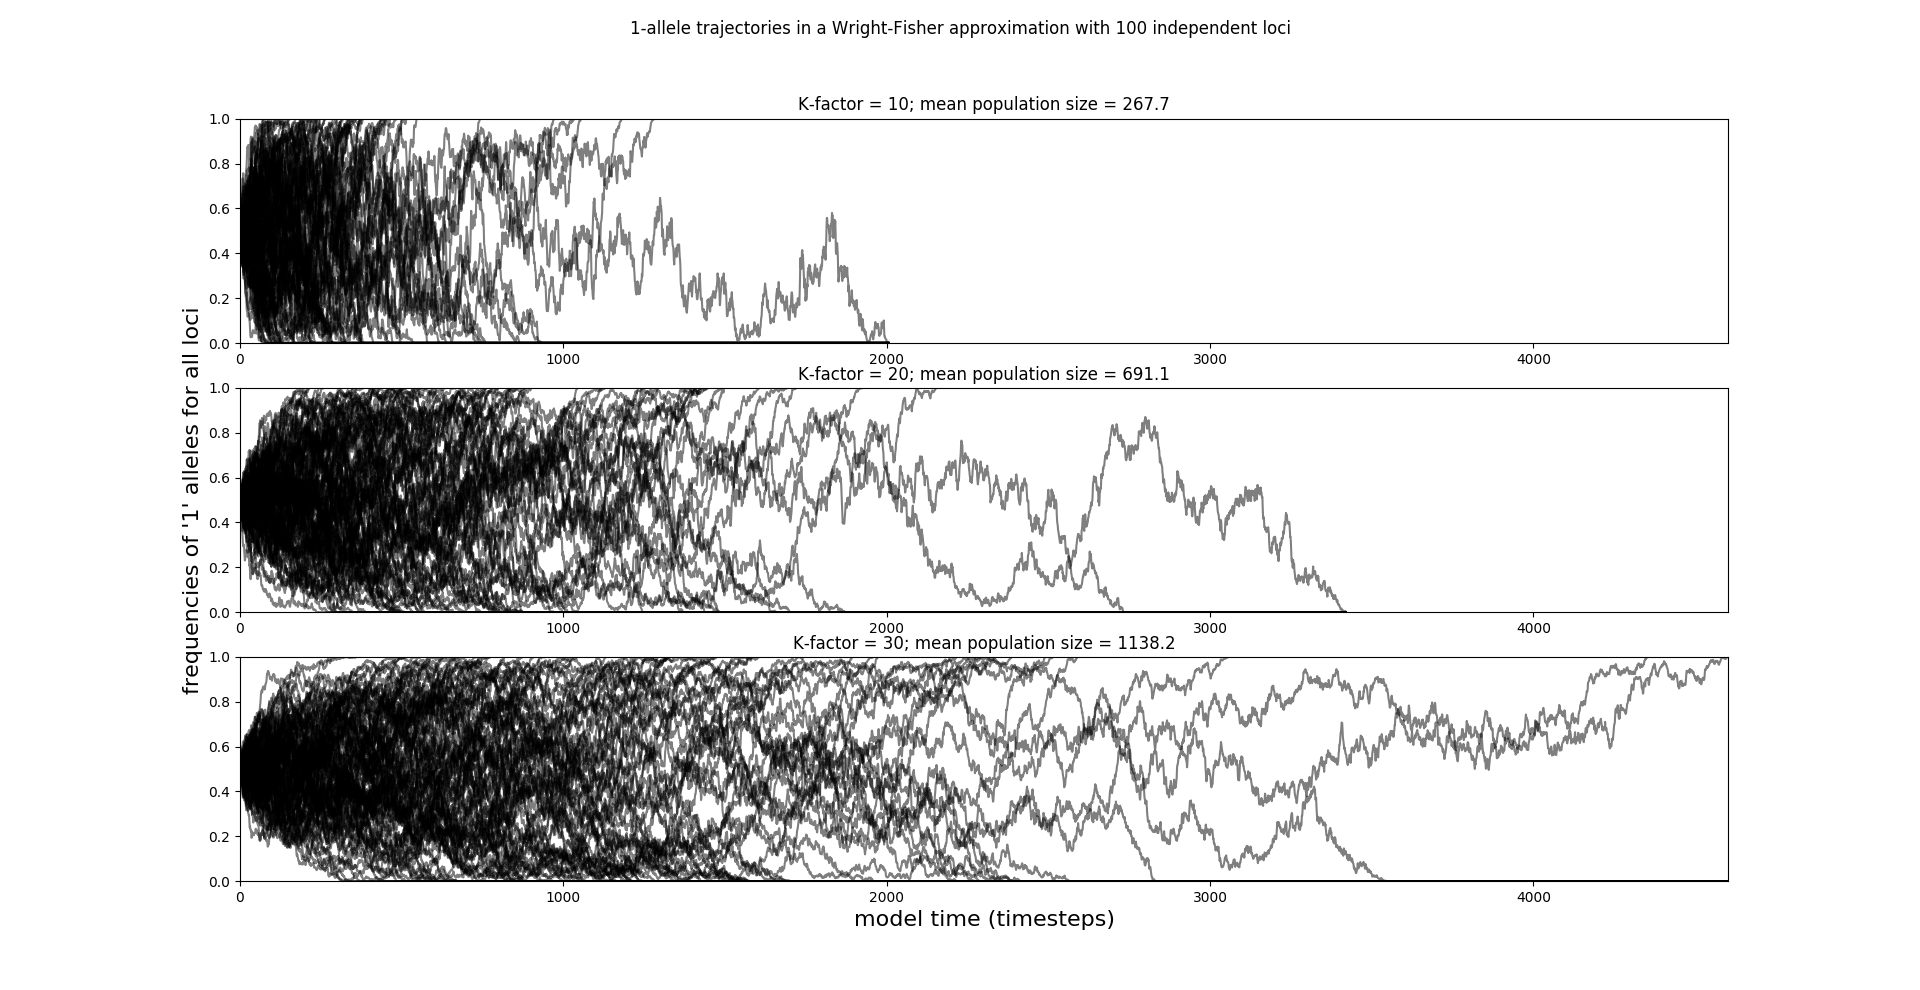
\includegraphics[width=175mm]{./img/validation/wf/allele_trajectories.png}
        \caption{Wright-Fisher test: allele-frequency trajectories}
\end{figure}

% fig 3
\begin{figure}[h!]
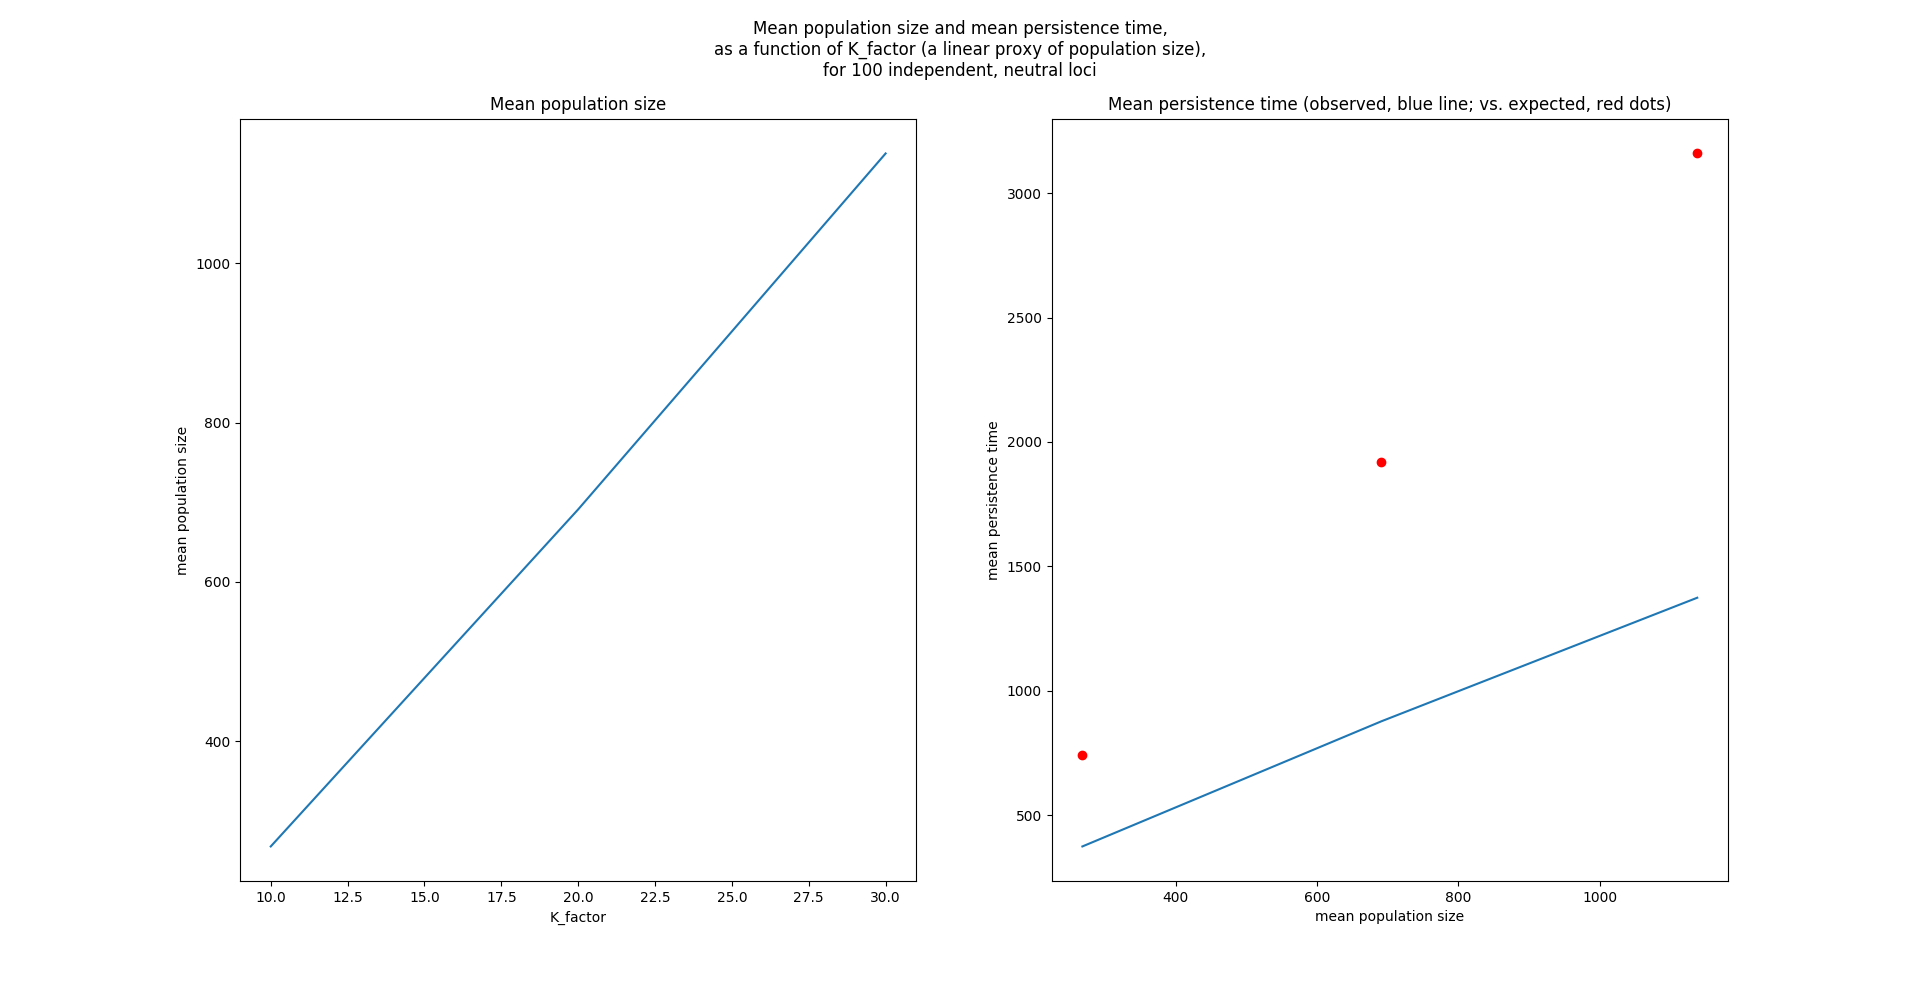
\includegraphics[width=175mm]{./img/validation/wf/pop_size_vs_K_factor_and_mean_persist_t_vs_pop_size.png}
        \caption{Wright-Fisher test: left: mean population size as a function of 'K\_factor' (multiplicative factor determining a species' spatialized carrying capacity and thus equilibrium population size; right: mean persistence time for segregating sites as a function of mean population size}
\end{figure}


\subsection{Bottleneck test: population dynamics}
Genetic drift is always operative in a population. Population dynamics can have
marked effects on the rate of drift; because drift is a stronger evolutionary
force in smaller populations, drift accelerates in shrinking populations. If a
population undergoes a sudden reduction in size, followed by a quick recovery to
its original size, i.e.\ a bottleneck event, the overall effect of drift on
that population is expected to be larger than a constant-size population of equivalent
starting size. In other words, the mean persistence time in that population
should be shorter in the bottlenecked population that in the constant-size comparison
population.

As with the Wright-Fisher model, I used a homogeneous landscape with broad distributions
for movement and dispersal and with a mating radius that encompasses the full landscape
to emulate aspatiality and panmixia. Geonomics features a variety of parameters for
parameterizing demographic change events. To simulate a bottleneck event,
I created a custom change event in which the population's carrying-capacity raster
is reduced to 30\% of its initial value for 50 timesteps (from the 200th to 250th),
then returned to its initial value for the remainder of the simulation
(through the 2500th timestep).
(I set other parameter values reasonably, or left them at defaults;
see \texttt{bottleneck\_params.py} for specifics.)


Figure 4 shows a clear signal of drift acceleration during the bottleneck event.

% fig 4
\begin{figure}[h!]
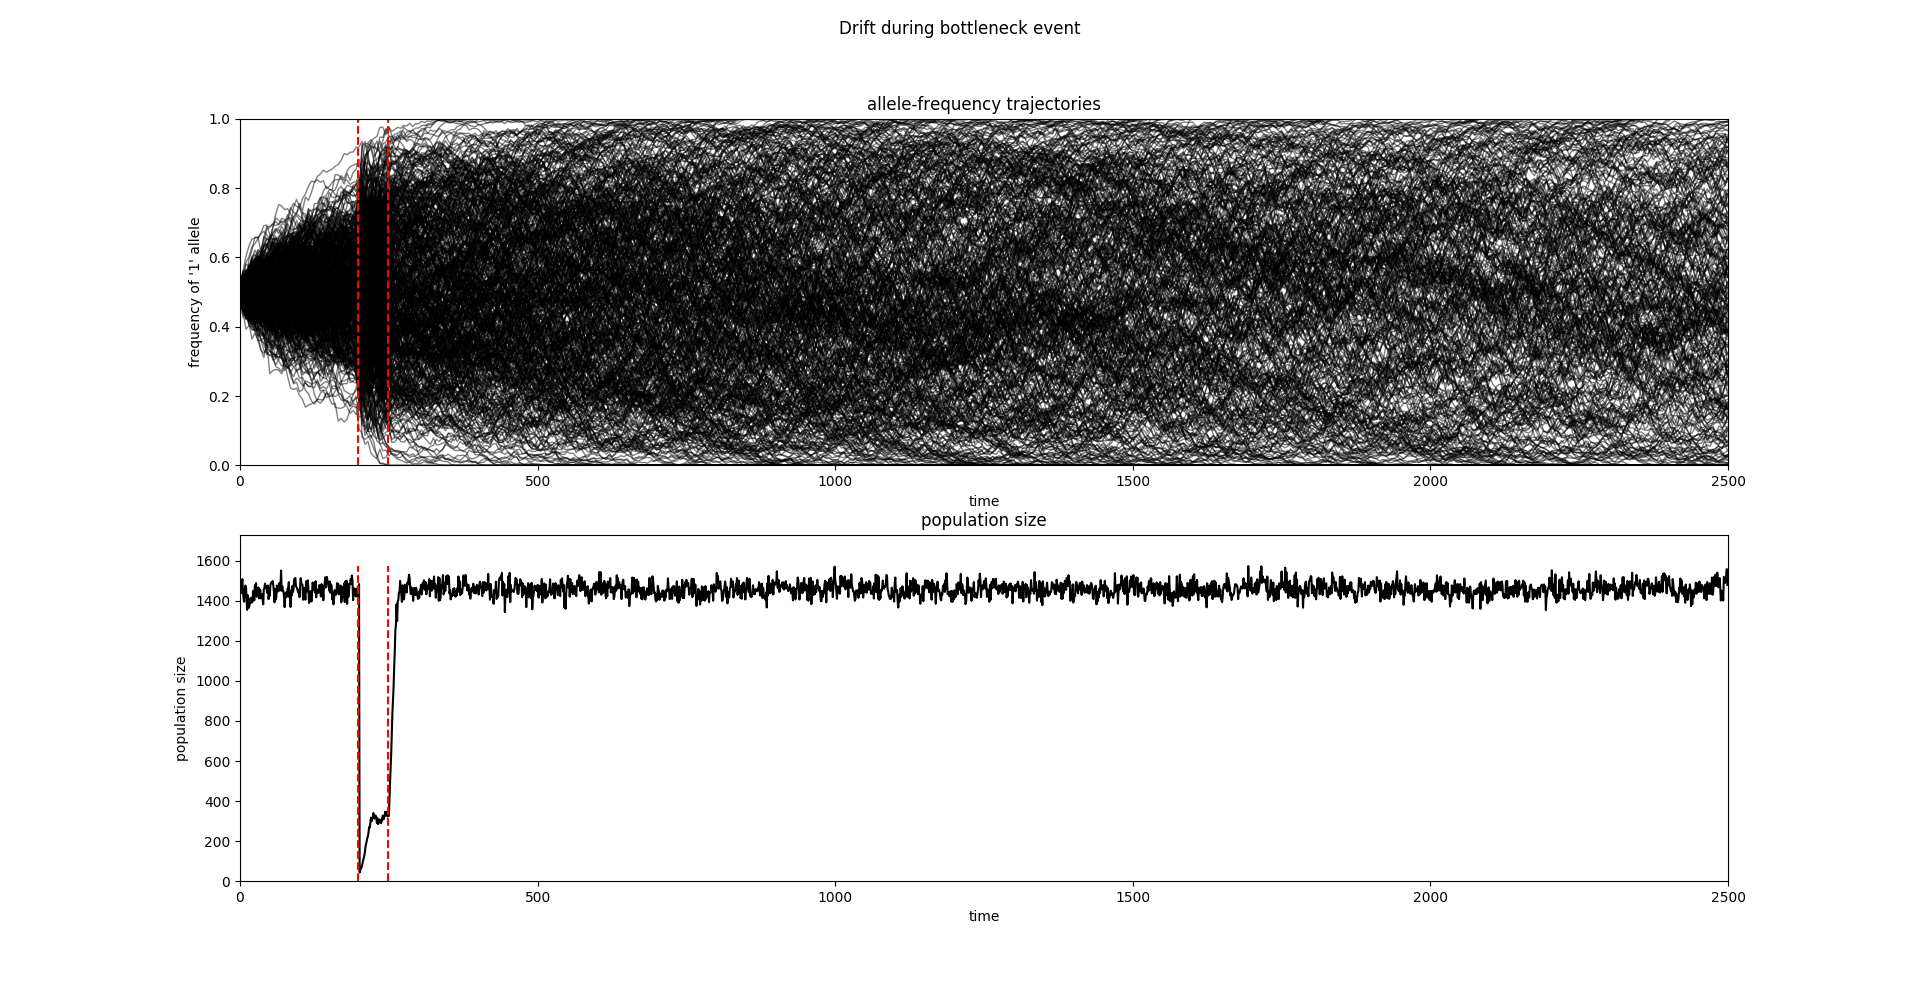
\includegraphics[width=175mm]{./img/validation/bottleneck/alleles_seem_to_take_too_long_to_fix.png}
        \caption{Bottleneck test: 1-allele frequencies (top) and population size (bottom) as a function of time}
\end{figure}


\subsection{Stepping-stone test: population subdivision and genetic differentiation}
The stepping-stone model, or one-dimensional island model, is a spatially implicit model.
It models a series of subpopulations, arranged along a straight line,
with migration between all neighboring pairs. (I chose to validate Geonomics using
the one-dimensional island model rather than the basic island model, in which all
island pairs have equal migration rates, because of the impossibility of arranging
more than three islands in two-dimensional space such that all island pairs are
equidistant, and thus have equal migration rates; this is fine, however, because for
the same reason it is unclear how applicable the basic island model is to real-world
systems.) As a combined result of divergence by drift and homogenization
by effective migration, subpopulations reach a stationary level 
of genetic differentiation---called migration-drift equilibrium. 
Theory provides the expected pairwise genetic differentiation
between a pair of subpopulations at migration-drift equilibrium
as:

\begin{equation}
F_{ST} = \frac{1}{1 + 4Nm}
\end{equation}

where $N$ is the population size and $m$ is the per-generation migration rate,
such that $Nm$ can be interpreted as the per-generation number of migrant
individuals {\large cite  Hartl and Clark 2007}

To approximate the stepping-stone model, I created a Landscape Layer with
a diagonal of six equally spaced islands (1.0-valued cells) embedded in 
a `sea' of 0.0-valued cells. I used this layer as the carrying-capacity raster. I set the
mating radius to encompass an individual's current island, but no neighboring islands. I
parameterized dispersal to be very local to parents' midpoints, and
parameterized movement to have a long right-skewed tail, such that long-distance movement
(and hence potentially migration) events are uncommon.
(I set other parameter values reasonably, or left them at defaults; see 
\texttt{stepping\_stone\_params.py} for specifics.) I ran the simulation for 5000 timesteps.
Because Geonomics cannot implement stipulated migration rates between
express portions of its continuous Landscape, I manually tracked the number of
migration events during each timestep, for all possible directional migration events 
(i.e.\ for all permutations of two islands). I used that data to solve the equation cited in the previous paragraph, and compared the resulting $F_{ST}$ expectations to the observed
values (calculated from the simulated date using two common methods;
see fig. 7 for details).

Results demonstrate that the model has approached reached migration-drift equilibrium
(fig. 5), and that all island populations were at dynamic equilibria around the
same mean size (fig. 6). Estimated migration rates and $F_{ST}$ values qualitatively
match theoretical expectations: islands greater than one step apart drop off 
precipitously and then continually decrease in mean migration rate,
and genetic differentiation increases toward a saturating level of $F_{ST}$.
Values of $F_{ST}$ consistently undershoot the values expected based on estimated
migration rates, however, likely because the subpopulations have yet to approach fixation
at most loci (i.e.\ the overall population has approached but still not reached
migration-drift equilibrium).

% fig 5
\begin{figure}[h!]
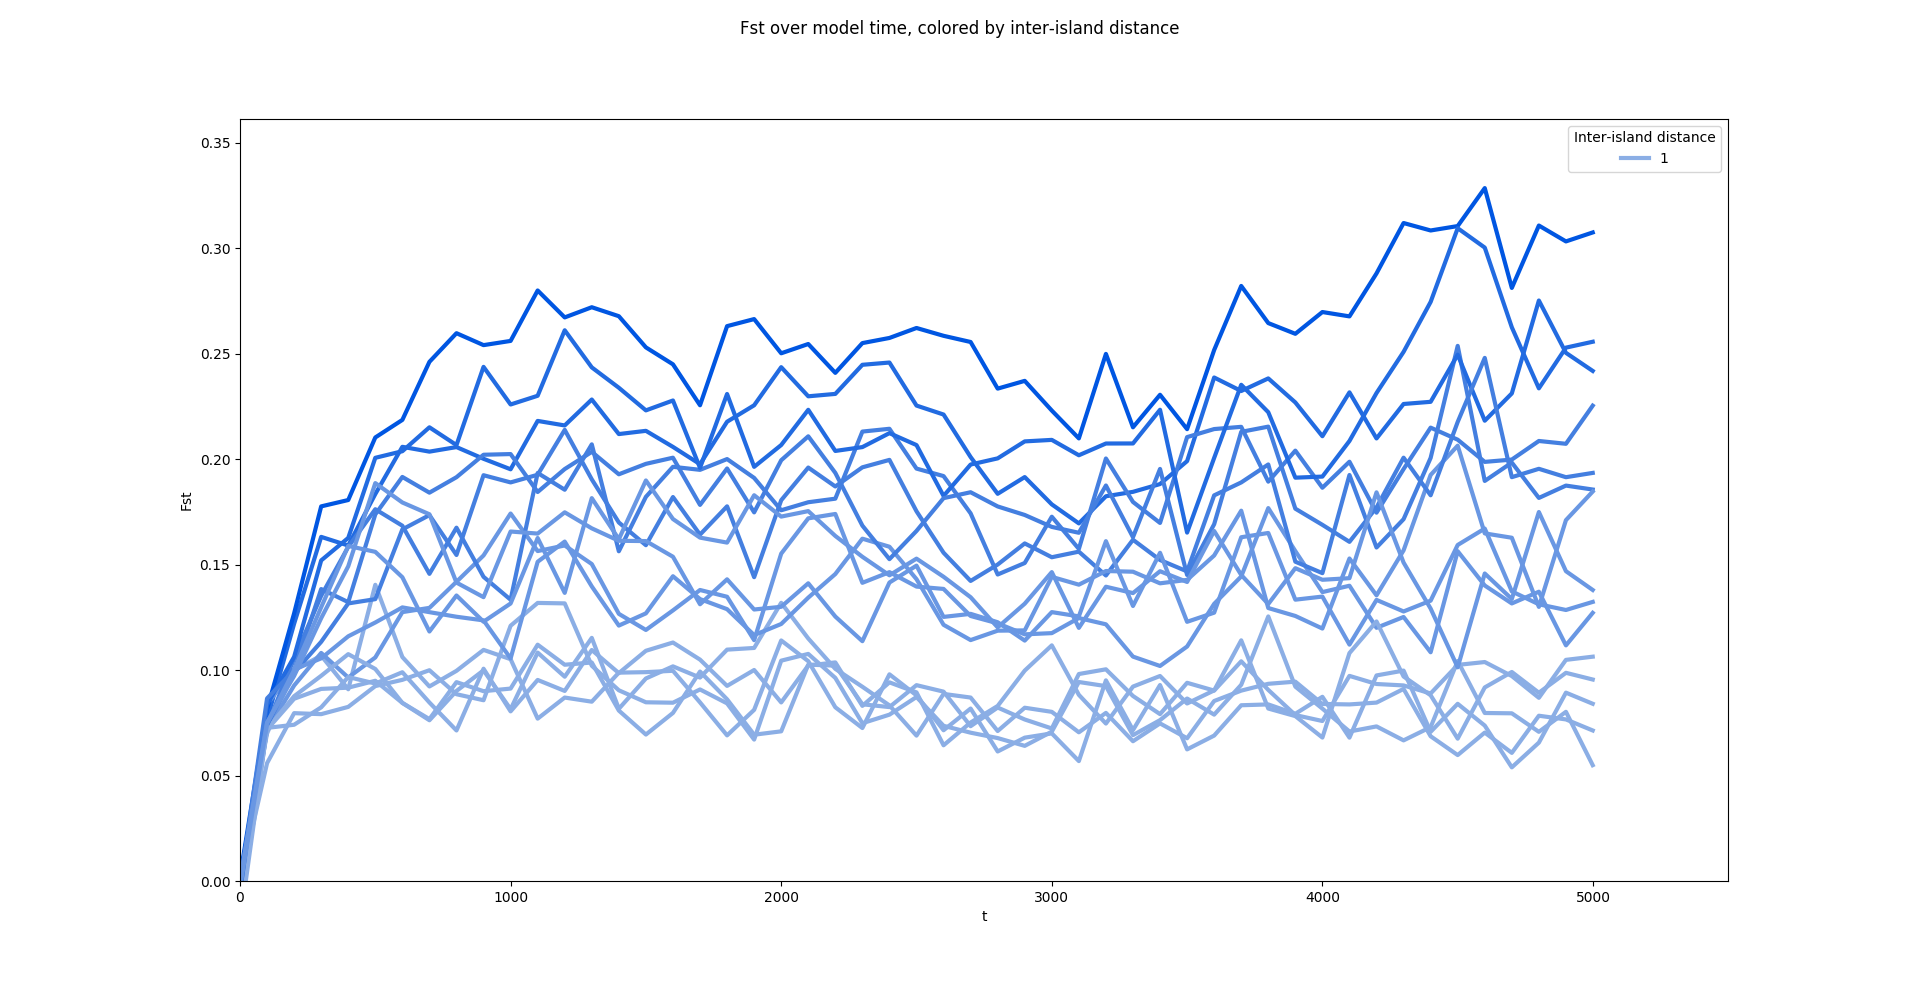
\includegraphics[width=175mm]{./img/validation/stepping_stone/Fst_over_time_vs_interisland_dist.png}
        \caption{Stepping-stone test: $F_{ST}$ as a function of model time, across increasing inter-island distances (gradually darker shades of blue)}
\end{figure}

% fig 6
\begin{figure}[h!]
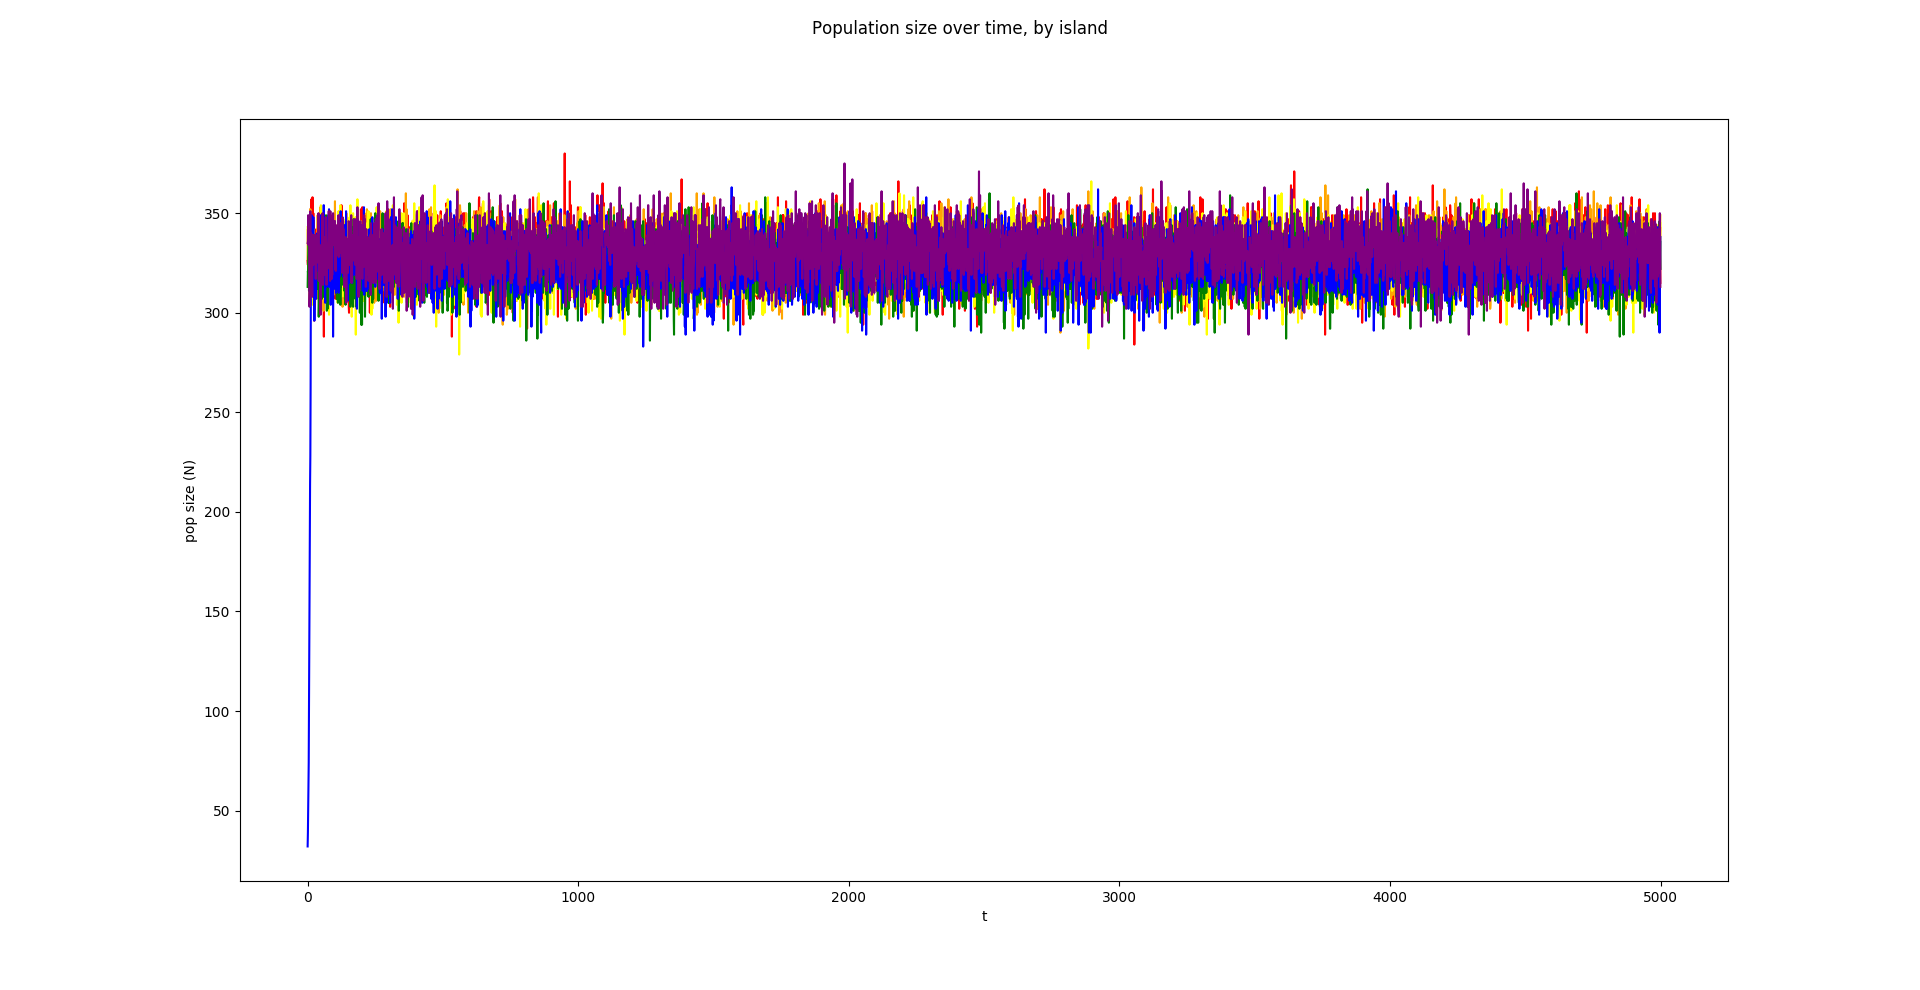
\includegraphics[width=175mm]{./img/validation/stepping_stone/pop_size_over_time.png}
\caption{Stepping-stone test: Population size as a function of time, for all 6 islands' populations}
\end{figure}

% fig 7
\begin{figure}[h!]
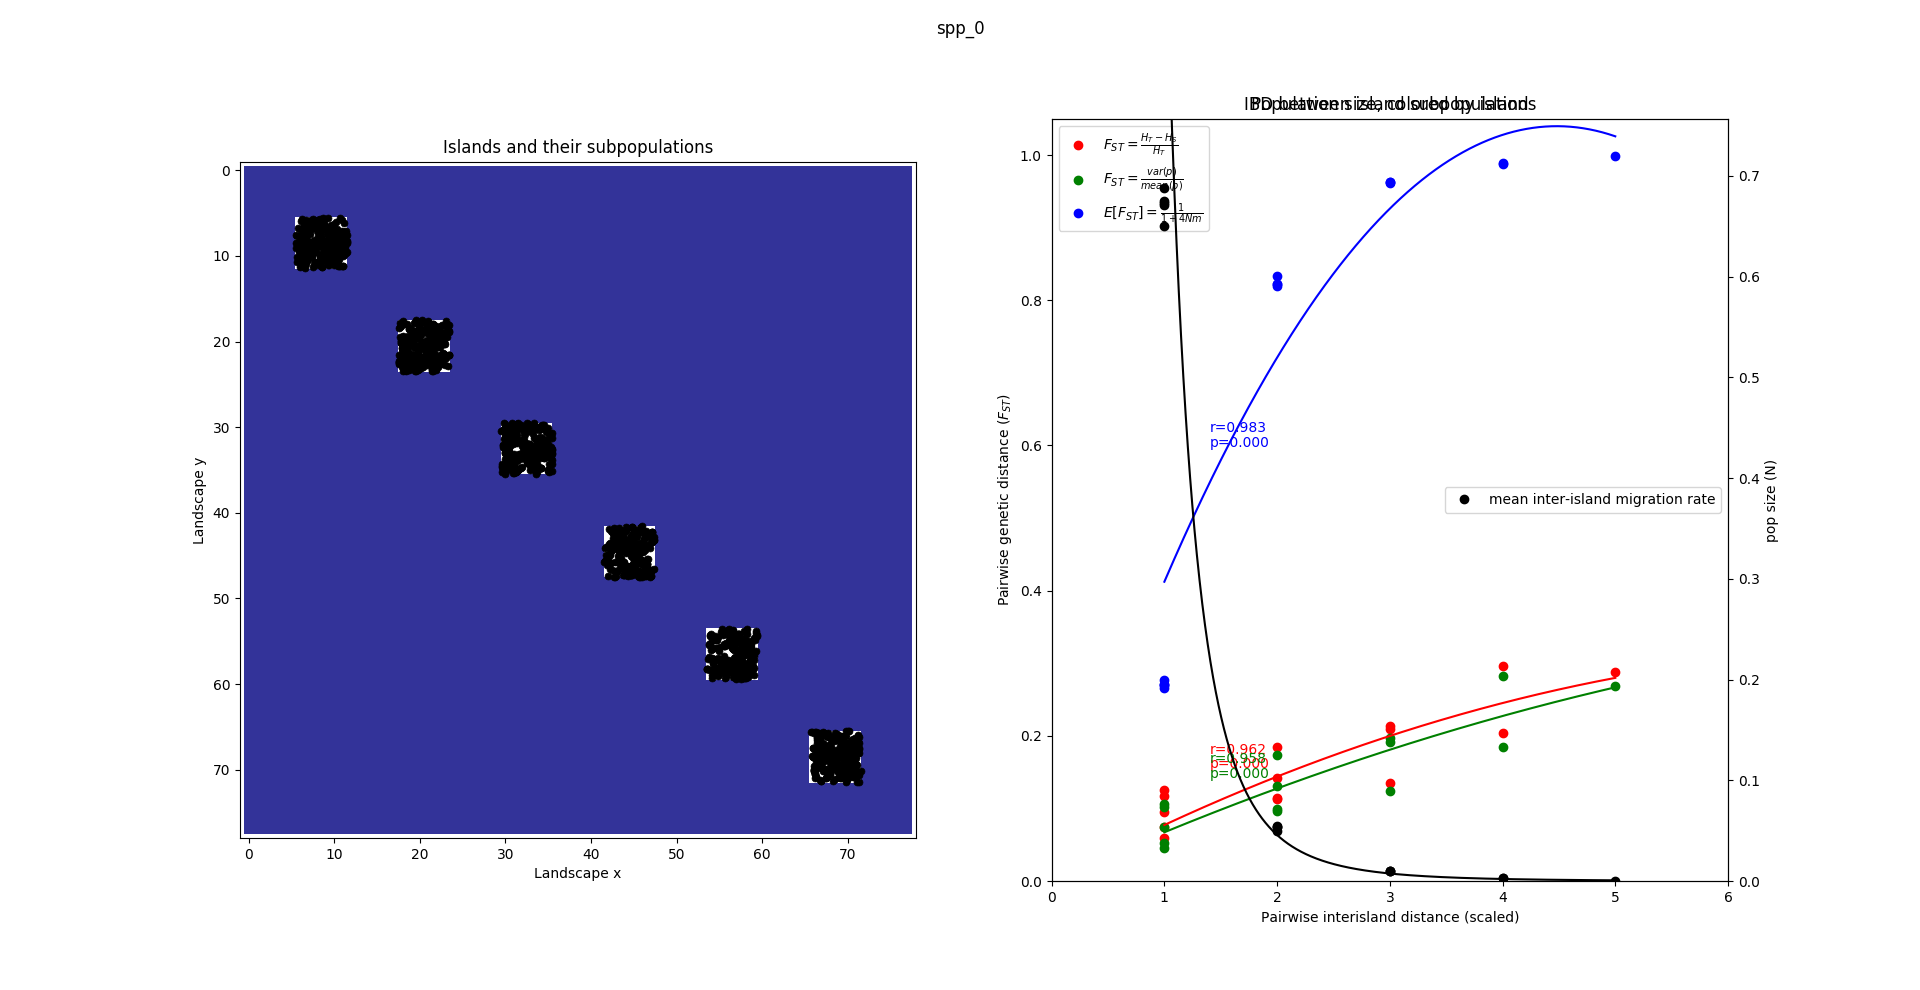
\includegraphics[width=175mm]{./img/validation/stepping_stone/pop_plot_and_Fst_and_mig_rate_plot.png}
        \caption{Stepping-stone test: left: Map of all 6 islands' populations at the end of the simulation; right: pairwise $F_{ST}$ (left y-axis; calculated by 3 different formulae) and inter-island migration rate (right y-axis) as a function of inter-island distance}
\end{figure}


\subsection{Contrasting-habitat test: adaptive divergence}
If a population is divided into two subpopulations which inhabit contrasting
environments exerting opposing selective forces, and there exists standing genetic
variation for a biallelic locus underlying a trait that is responsive to those
selective forces, then theory predicts that the two subpopulations will diverge at
that locus as each population moves toward its respective adaptive peak. Analogously
to the stepping-stone model, the rate at which that divergence will occur,
in each of the subpopulations, depends on the relative strengths
of two opposing evolutionary forces: the strength of natural selection,
which causes divergence, and the strength of gene flow from migration,
which homogenizes the two subpopulations. The rate of allele frequency change
in either subpopulation at timestep t is expressed as:

\begin{equation}
\delta{q} = \frac{-spq[q + h(p - q)]}{1 - sq(2hp + q)} + m_{i}q^{*} - m_{o}q
\end{equation}

where $q$ and $p$ are the frequencies of the deleterious and beneficial
alleles (with respect to the subpopulation being analyzed), $s$ is the selection
coefficient against the homozygous recessive phenotype, $h$ is the degree of dominance
of the recessive allele, $m_{i}$ and $m^{o}$ are the migration rates into and out of
the subpopulation being analyzed, and $q^{*}$ is the frequency of the recessive allele
in the alternative subpopulation {\large cite Hartl and Clark 2007}.

This model, much like the stepping-stone model, is spatially implicit
(except in cases where it is used to represent sympatric ecological isolation).
To approximate this, I created a Landscape with two Layers. The first
was divided into two equal-sized halves, valued at 0.0 and 1.0, and was used
as the environmental variable driving natural selection (such that 0.0 and 1.0
phenotypes were most fit, respectively). The second was valued uniformly at 1.0,
and was used as the habitat-quality layer, which served as the carrying-capacity
raster (thus setting uniform population density across the Landscape and determining,
in sum, the overall carrying capacity of the landscape).
I created one monogenic trait whose locus was randomly chosen within a 
genomic architecture of 100 independent (i.e.\ unlinked) loci. This trait was selected
upon the first landscape layer.  (I set other parameter values reasonably, or left them
at defaults ;see \texttt{divergence\_params.py} for specifics.) I ran the model for 1000
timesteps for each of three values of phi (which for a monogenic trait is
identical to \emph{s}, the selection coefficient in classical population genetics): 
0.1, 0.05, and 0.01. Given that Geonomics does not employ express migration rates,
I tracked the number of migration events during each timestep and used that
data to solve the equation cited in the previous paragraph.

Results depict clear local adaptation to each of the two halves of the landscape,
with opposite-phenotype bleedover and heterozygote births occuring mainly along
the border between the two habitats (fig. 8, right).
Allele trajectories in each half of the
environment follow qualitatively the increasing and saturating trajectories expected by
theory, but reach consistently more extreme allele frequencies than expected (fig. 8,
left). This is likely because of WHAT?

% fig 8
\begin{figure}[h!]
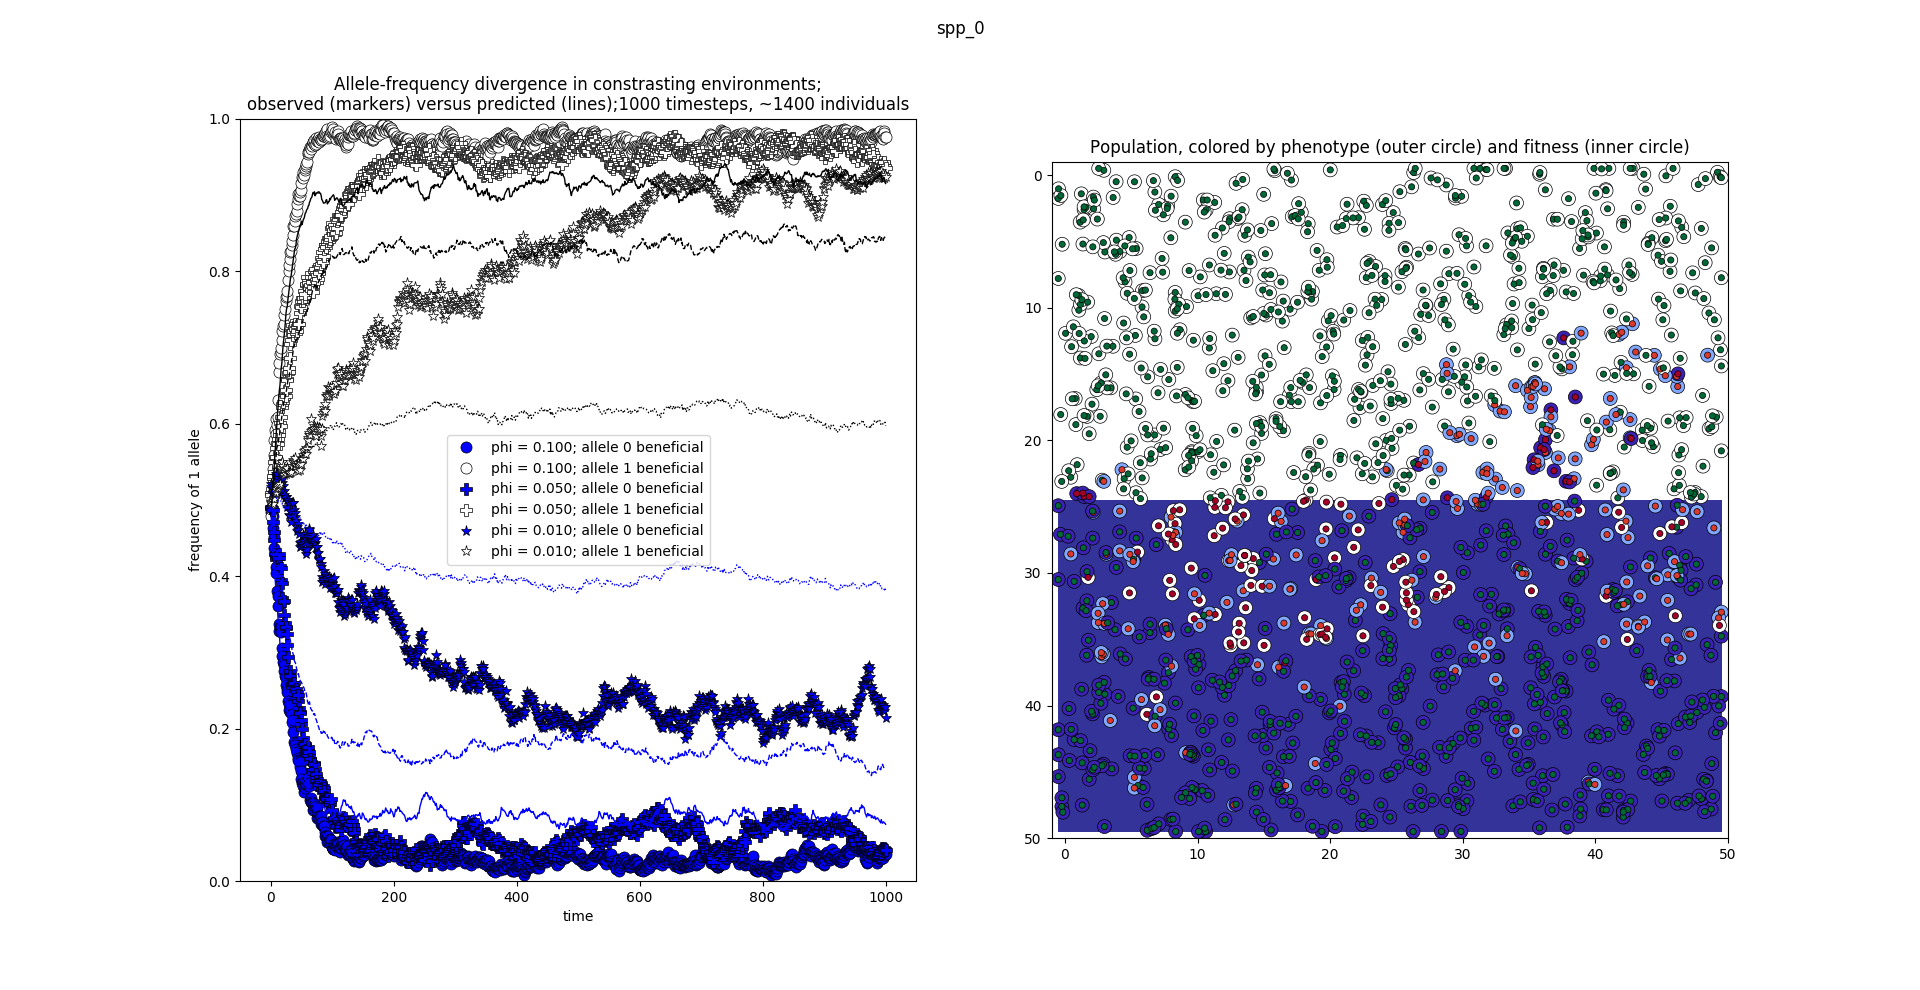
\includegraphics[width=175mm]{./img/validation/divergence/divergence_test_ca1400_individuals_1000_timesteps.png}
        \caption{Contrasting-habitat test: left: Observed (markers) versus predicted (lines) allele-frequency trajectories for two contrasting habitats (blue = 0.0-valued; white = 1.0-valued), across three selection coefficients ($\phi$ = 0.01: stars; 0.05: crosses; 0.10: circles); right: map of the population after spatially divergent selection at $\phi$ = 0.10, with individuals, colored by phenotype (outer circles) and fitness (inner circles), plotted on top of the selective landscape layer (horizontally divided into white and blue halves)}
\end{figure}


\subsection{Cline test: local adaptation}
Similar to the contrasting-habitat model of adaptive divergence, but perhaps more
to most real-world cases of local adaptation, is the cline model. In this model,
a population adapts locally across a continuous environmental gradient,
which is characterized by the extremes of its environmental values and its steepness
(i.e.\ the instantaneous rate of environmental change along it). Local adaptation
across this gradient will generate a cline, i.e.\ a geographic gradient in allele frequency
(though of course natural selection is not the only evolutionary force that can
generate a cline). In the clinally adapted population, loci that underlie the trait
undergoing clinal selection are expected to exhibit clinal variation in allele frequency
that mirrors the environmental gradient driving selection, whereas loci unlinked to 
those loci have no long-term expectation of concordant clinal variation (though they could
initially be swept along with the selective locus if the beginning stages of clinal
adaptation, and any number could continue to show spurious concordant clinal variation
by chance). To detect clinally adapted loci, we can fit cline curves to the spatial
allele-frequency variation at all loci, with the expectation that the clines fit to
adaptive will match the environmental gradient. Numerous equations have been used
to fit clines, but classical models include a sigmoidal \emph{tanh} function
of the following form:

\begin{equation}
p_{x} = \frac{1}{2}(1 + \tanh[\frac{2(x - c)}{w}])
\end{equation}

where $p$ is the frequency of the reference allele at position $x$ along the cline,
$c$ is the centerpoint of the cline (such that $p_{x=c} = 0.5$), and $w$ is the 
`width', which is defined as $w = \frac{1}{slope}$ at centerpoint
$c$ {\large cite Porter ClineFit manual}.

To implement the cline model in Geonomics, I created a landscape with two layers.
Similarly to the landscape used in the divergence model (see previous section), the
landscape consisted of two layers, the first being an environmental layer (in this case a
symmetrical non-linear gradient between 0-valued and 1-valued halves, rather than two
discrete 0- and 1-valued halves), the second being a uniformly valued
habitat-quality layer (used to set a uniform population density and thus determine
the global carrying capacity). Also similarly to the divergence model, I created a
monogenic trait whose locus was randomly placed within a genomic architecture of 
100 independent loci. The trait had a \emph{phi} (i.e.\ \emph{s}) of 0.01,
and was selected upon by the gradient layer.
(I set other parameter values reasonably, or left them
at defaults; see \texttt{divergence\_params.py} for specifics.)

I ran the cline model for 2500 timesteps, then used a numerical optimization
function in Python's \texttt{scipy} package to fit \emph{tanh} clines to all loci.
I plotted all fitted clines on top of the first landscape layer, with the cline
for the one selective locus highlighted.
The selective locus consistently and clearly stands out as the only locus with a cline
matching the expectation (i.e.\ mirroring the environmental gradient; fig. 9, left),
and results show an obviously locally adapted population, with a zone of hybridization
and phenotypic spillover surround the clinal center (fig. 9, right).
Furthermore, for a family of regression models of environmental value on genotype
for all loci, after correction for multiple testing, the selective locus consistently
stands out as the most significantly correlated locus (though numerous other loci
also give false-positive results, albeit with considerably larger p-values). SHOW
THESE RESULTS!

% fig 9
\begin{figure}[h!]
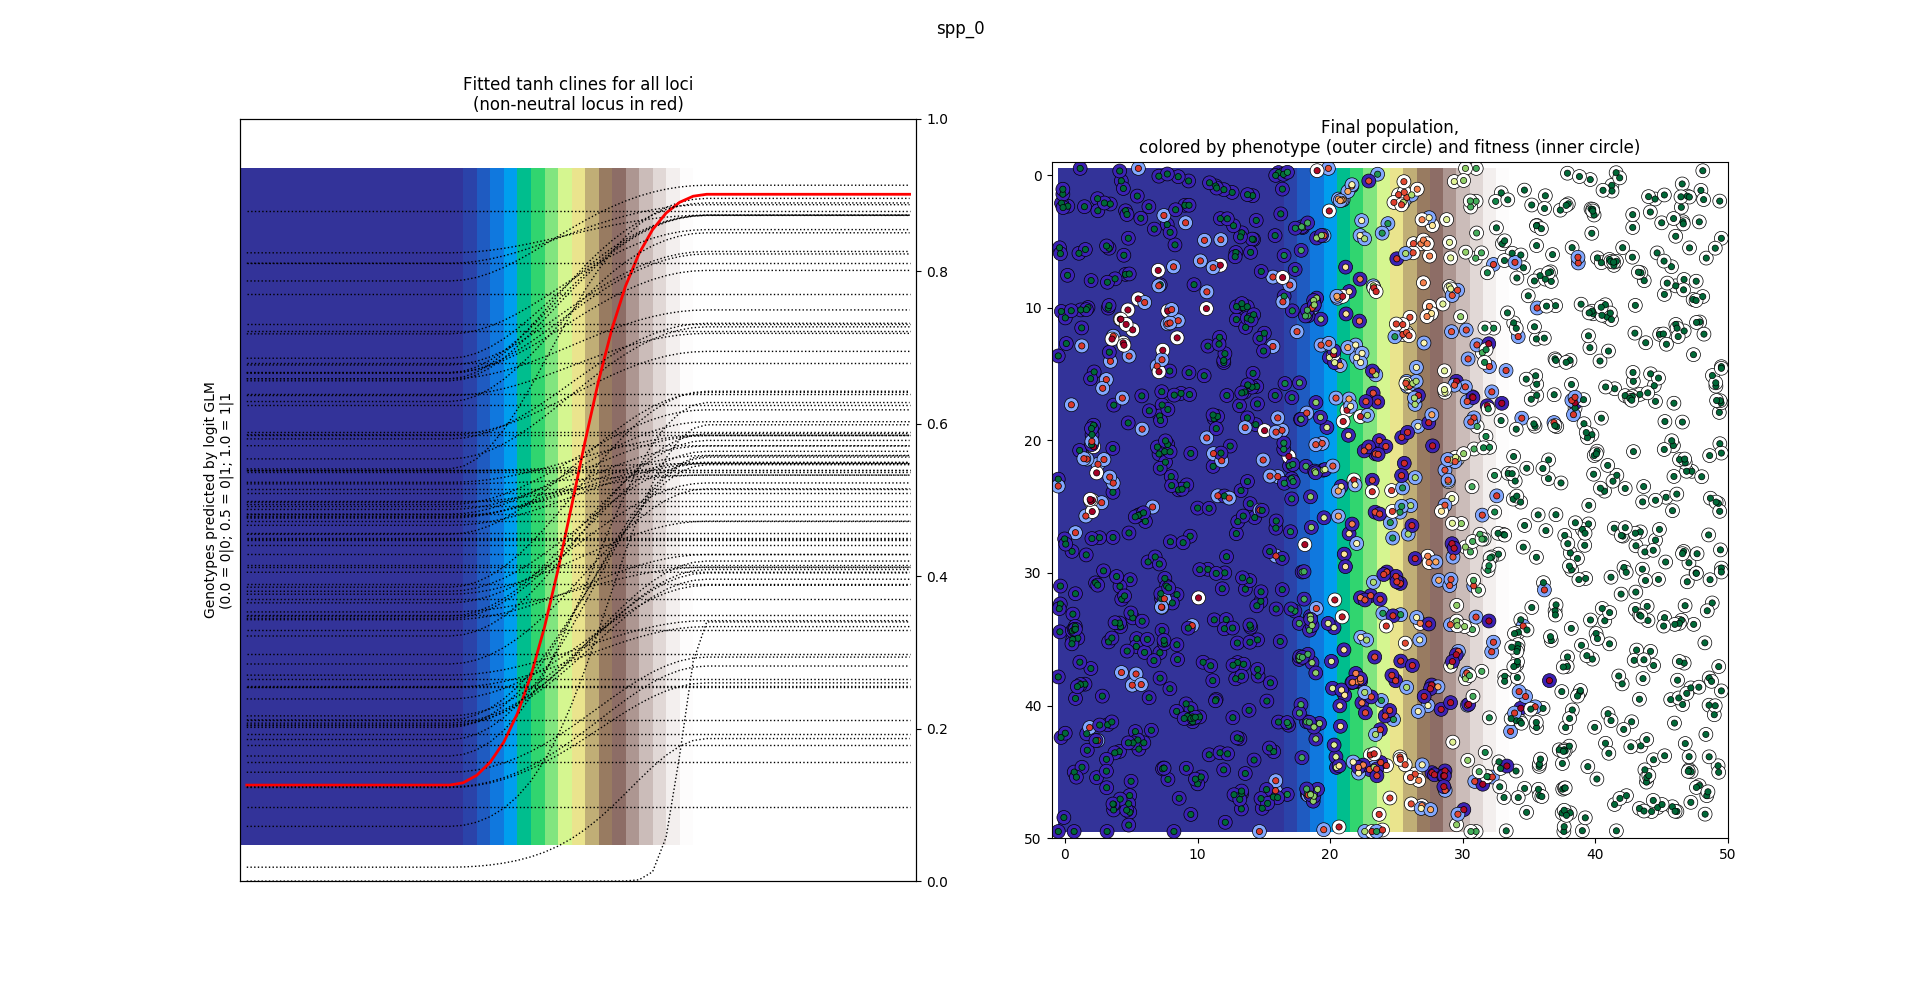
\includegraphics[width=175mm]{./img/validation/cline/cline_adaptation_phi_0pt01_2500_timesteps.png}
        \caption{Cline test: left: plot of allele-frequency clines (neutral loci in black, selective locus in bold red) against the selective landscape layer (horizontal gradient from blue to white); right: map of the final population on top of the selective lanscape layer, with individuals colored by phenotype (out circles) and fitness (inner circles)}
\end{figure}


\subsection{Selective sweep test: genetic hitchhiking}
While classical population genetics provides us with a great
deal of understanding under scenarios of selection 
on unlinked loci, population genomics attempts to reckon
with the reality that all loci under selection are actually
embedded within a contiguous genome, and thus are tightly linked
to a block neighboring loci. Consideration of genomic context and linkage
considerably complicates the study of molecular adaptive evolution, but is
essential for understanding and interpreting data in the genomic age. The
most basic model of selection with linkage is that of the selective sweep:
a beneficial mutation occurs in a population, falling on a
random genomic background, and then rises in frequency because of its
selective advantage until it becomes fixed, pulling up the frequency of its
haplotype as it does so. But even as the haplotype increases in frequency it is
continually subject to recombination, which gradually erodes the haplotype block,
causing it to contract around the beneficial mutaiton and freeing its
loci from linkage to the mutation. Thus the model predicts that once a
beneficial mutation occurs---as long as it is not lost early on by chance---
it and a haplotype block around it will rise in frequency, the mutation will
eventually fix, and the haplotype block will continually fade over time.
The haplotype block should be clearly visible in genomic data, where it will
manifest as a genomic region of reduced diversity and heterozygosity, centered
on the mutation.

To implement the selective sweep model in Geonomics, I again created a model
approximating an aspatial, panmicitic population (with movement and dispersal
distributions and mating-radius broadly encompassing the landscape, as for
the Wright-Fisher and bottleneck tests, above).
I created a single, monogenic trait in this population, with a \emph{phi} of
0.15, and with its locus manually set to 50, and thus centered
within the 101-locus genomic architecture. I manually set the starting 
'1'-allele frequency at this locus to 0.0, but set the trait to selected upon
by the landscape's first and only layer, a uniformly 1-valued raster, such
that all individuals began the model equally ill-fit (i.e.\ with a fitness value of
$1 - \phi = 0.85$). I burned the model in. Then I iteratively chose a random individual,
introduced a '1'-mutation in their genome at locus 50, ran the model for 50 timesteps,
and checked whether the '1' allele had reached a frequency greater than 0.05 by that
time. I iterated until that check was passed, at which point I declared
the mutant allele `established' and continued to run the model until 2500 timesteps
after the mutant allele had fixed, calculating genome-wide nucleotide diversity
at three points during the model.

Geonomics very realistically emulated the behavior of a selective sweep. The
adaptive phenotype (the '1'|'1' genotype, plotted as white
on a white environmental background; in fig. 10, top row) clearly
emerges in a region surrounding the mutation's origin, then spreads rapidly
throughout the population from there. The population's mean fitness increases
quickly from 0.85 (the universal fitness value before the mutation is
introduced) to 1.00 (the universal fitness value after the sweep is complete;
fig. 10, bottom row, leftmost plot). And there is a clear region of depressed
nucleotide diversity immediately around the selective locus, which becomes
more pronounced once the sweep goes toward completion, then slowly erodes
over further time as a result of recombination of the mutant haplotype's
alleles onto non-mutant backgrounds (fig. 10, bottom row, second, third, and
fourth plots from the left).

% fig 10
\begin{figure}[h!]
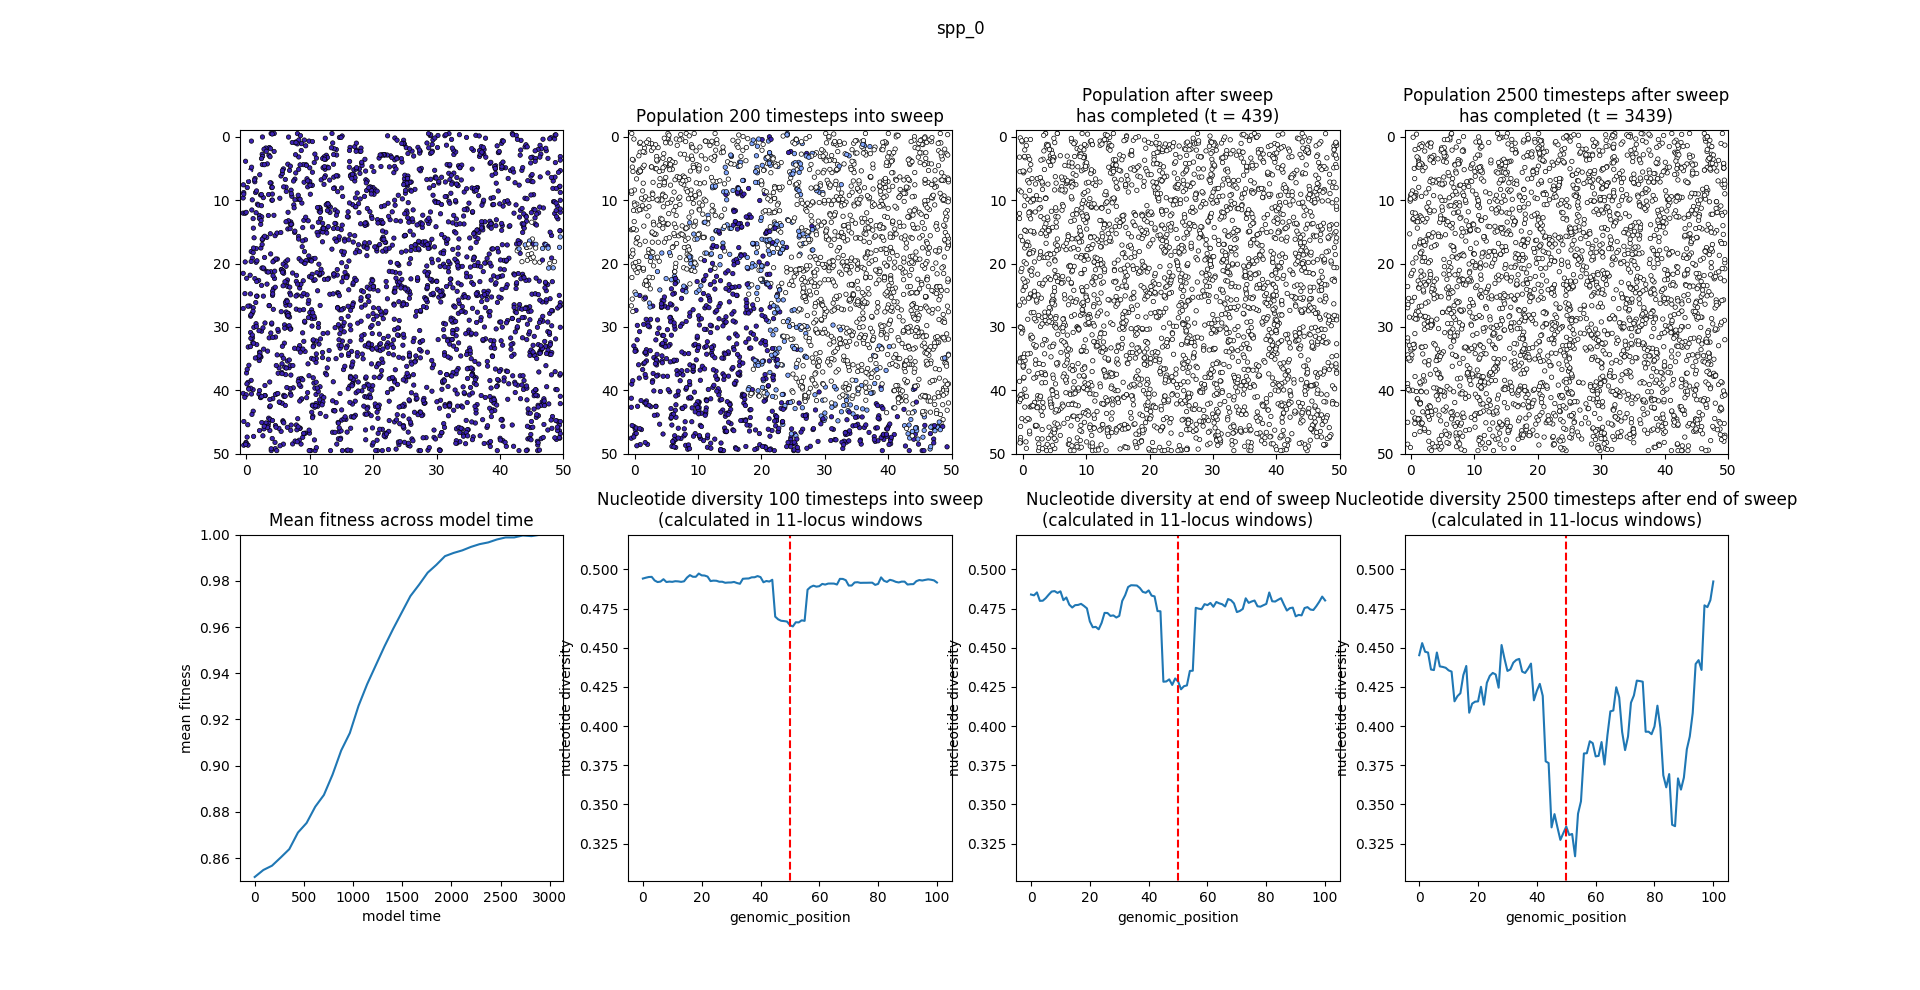
\includegraphics[width=175mm]{./img/validation/sweep/sweep_results.png}
        \caption{Selective sweep test: top row: Maps of population (colored by phenotype) at various points in model time (from left to right: timestep 0, timestep 200, after completion of sweep, and 2500 timesteps after completion of sweep); bottom row: mean fitness as a function of model time (first plot on left) and genome-wide nucleotide diversity at timestep 200, immediately after completion of sweep, and 2500 timesteps after completion of sweep (second, third, and fourth plots from left)}
\end{figure}


\section{Example use-case: Polygenic adaptation to climate change in the Yosemite region}

Perhaps Genomics' use-value is best demonstrated by way of a worked example.
In this section, I explain a complex evolutionary scenario for which 
simulated data is desirable, explain the steps by which I have simulated the
scenario in Geonomics, and present the simulation results. (The source code for
this example is available within the \texttt{./example/yosemite} directory
of the Geonomics repository.)

There is growing interest in the evolutionary implications of climate change.
Much of this interest focuses on species that are locally adapted along some
environmental gradient that is expected to shift, perhaps non-linearly,
under climate change, and particularly with the potential for such species
to respond adaptively to the change.

Here I simulate an example of such a study system: the adaptive
response of a continuously disributed, locally adapted species
to non-linear climate change in the Yosemite region. To begin with, I have
downloaded a raster dataset of 30-year temperature normals of the Yosemite
region (from Cal-Adapt; \url{www.caladapt.org}), cropped it to a 90-cell by
90-cell window around the Yosmite valley, and saved the cropped file. I then
wrote a couple quick functions to process that raster into the full set of
rasters I needed for my simulation.

Temperature is the environmental variable driving natural selection.
In order to model adaptive responses to change in this variable, I needed
a raster of future temperatures, to feed into a landscape-change event
as the endpoint raster.
(I could have downloaded a series of future-projection rasters, and loaded
them in as the stepwise changes for the environmental-change event that I will
create in this Geonomics model, because Geonomics is designed to accept a
directory of such files as the steps in a change event. However, to keep
things simple I just processed the 30-year normals raster with a simple,
heuristic function.) So I wrote a function that adds to the 30-year normals
raster a fixed temperature increase (2 degrees) plus an additional,
elevation-dependent fraction of that increase (where there fraction varies
from 0.0 at the hottest cell to 1.0 at the coldest cell). This function
emulates the fact that warming due to climate change appears to be quickest
at high elevations. I saved the resulting future-temperature array to a new
raster file.

I also needed habitat-quality rasters for the model. These should reflect
the fact that species tend to find highest-quality habitat, and thus exist at
their highest densities, in the core of their range, and that edge habitat
becomes increasingly marginal. Thus I wrote a function that accepts the
temperature raster as input and produces from
it a second, core-edge-type habitat-quality raster (where cells with
temperature values between 7 and 11 degrees are assigned a 1.0 quality value,
and cells outside that range are assigned quality values that linearly decrease
to 0.0 in the hottest and coldest cells in the raster). I fed both the 30-year
normals raster and the future temperature raster through this function, thereby
generating both current and future habitat-quality rasters, which I saved to
new raster files.

With these rasters prepared, I then created a Geonomics parameters file.
I needed to parameterize a model with 2 `file'-type Layers,
both of which would undergo landscape-change;
with 1 Species, with movement, a movement-surface, and
genomes with 1 trait; and with data-collection.
The command to do this was:

\begin{allintypewriter}
>>> gnx.make\_parameters\_file(filepath=`yosemite\_params.py',\\
                               layers=[\{`type': `file', `change': True\},\\
                                       \{`type': `file', `change': True\}],\\
                               species=[\{`movement': True, `movement\_surface': True,\\
                                          `genomes': True, `n\_traits': 1\}],\\
                               data=True)\\
\end{allintypewriter}

After running this command, I opened the resulting, auto-generated parameters
file (\texttt{yosemite\_params.py}) and edited the parameters as needed. In the Layer
`init' and `change' parameters secitons I replaced
the placeholder filenames with the names of the four temperature-derived
rasters whose creation I explained above. I parameterized my landscape-change
events: both Layers would change from their original rasters to their final
rasters in 20 stepwise changes over 1000 timesteps (i.e.\ 1000 years),
starting on timestep 499 and finishing on timestep 1499. The habitat-quality
layer would serve as the basis for the movement-surface. The model would include
no mutation. I stipulated the selection coefficient (\emph{phi}) on my trait
(0.05), and the number of loci underlying it (100 randomly-selected loci).
Other parameters were left at default values.

Finally, I wrote a short script to create a model from the parameters 
(`mod = gnx.make\_model('./yosemite\_params.py')`), and then to manually
burn in and run the model (by using the \texttt{mod.walk} function to run the model
in either `burn' or `main' mode for the desired number of timesteps, and using
\texttt{mod.plot\_<\_>} functions or manual \texttt{matplotlib} code
to plot the model at various timesteps during its progress).

The model generates a clear and realistic pattern of polygenic adaptation to
the elevation-based temperature gradient in the Yosemite region, and that
gradient of local adpatation exhibits a pronounced upslope shift in response to
the period of climate change. These results are visible both heuristically
(from the individuals' phenotypes plotted across the three discrete timesteps'
columns in fig. 11) and analytically (from the neighborhood-meaned phenotype
rasters plotted across fig. 11, row 3).

% fig 11
\begin{figure}[h!]
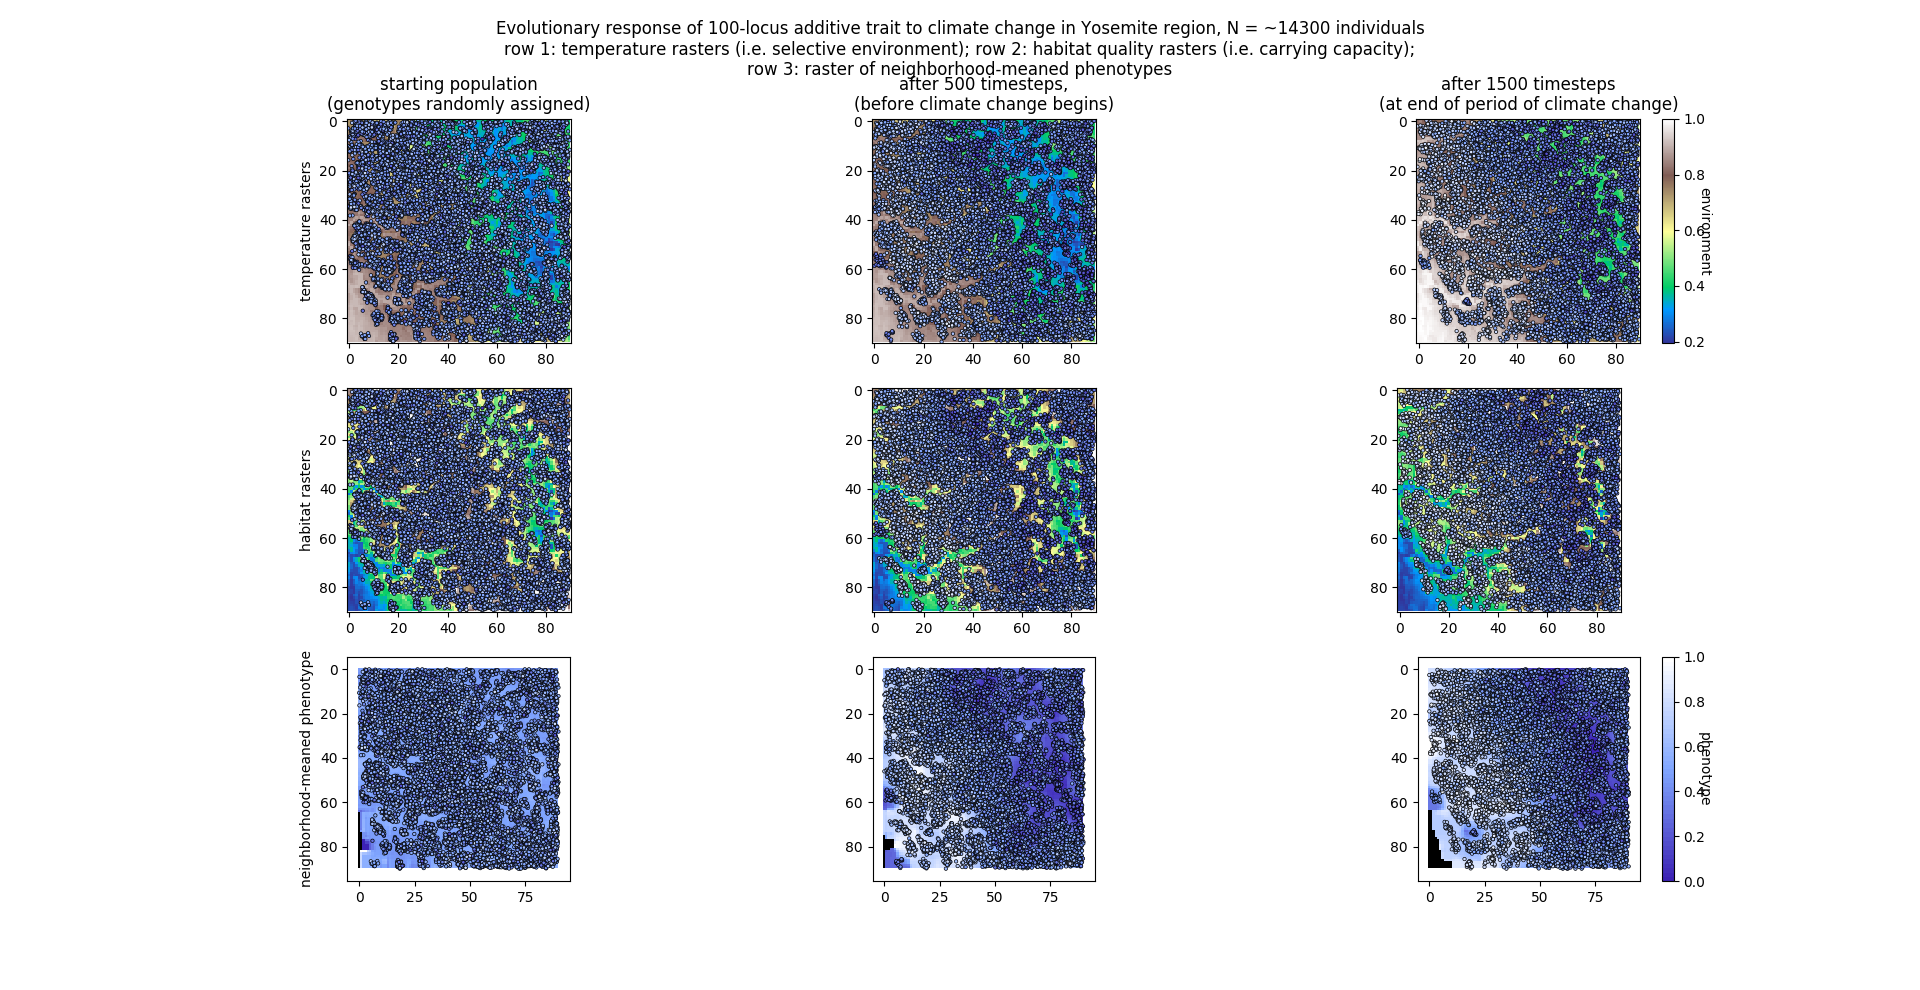
\includegraphics[width=175mm]{./img/example/yosemite_results.png}
        \caption{Temperature rasters (top row), habitat rasters (middle row), rasters of neighborhood-meaned phenotype (bottom row) at timesteps 0 (left column), 500 (before beginning of climate change; center column), and 1500 (after climate change; right column) for a species with a 100-gene trait adapted to temperature}
\end{figure}


\section{Getting started}
For those interested in using Geonomics, the simplest way is to install
via \texttt{pip} (the most popular Python package-installation software),
by calling \texttt{\$ pip install geonomics}.
(Note that Geonomics only uses common, well established Python packages
as required dependencies: \texttt{numpy} \texttt{matplotlib},
\texttt{pandas}, \texttt{shapely}, \texttt{bitarray}, \texttt{random},
\texttt{scipy}, \texttt{sklearn}, \texttt{statsmodels}, and \texttt{vcf}.)
The source code is also publicly available on GitHub (\url{URL_HERE}),
where it is actively maintained and developed.

Documentation is extensive (and continues to expand as new worked examples
are offered and new functionality is added to the package), and is available
online at \url{http://htmlpreview.github.io/?https://github.com/drewhart/geonomics\_docs/blob/master/built/doc.html}.  
The simplest and advanced use cases are explained above (see section
\emph{Design, structure, and function}), as well as in the documentation.
The documentation provides a detailed section explaining the meaning,
default values, and usage for every parameter in a Geonomics parameter
file.
Both the documentation and specific functions' docstrings (available
by calling Python's \texttt{help()} on the function of interest) provide
details on the usage of each function.

\section{Works Cited}


\end{document}
